% Compile with: xelatex npm_paper_CN_v13.tex
\documentclass[11pt,a4paper]{article}

\usepackage[margin=1in]{geometry}
\usepackage{amsmath,amssymb,amsthm}
\usepackage{booktabs}
\usepackage{graphicx}
\usepackage{hyperref}
\usepackage{xcolor}
\usepackage{xurl}
\usepackage{enumitem}
\usepackage{float}
\usepackage{authblk}
\usepackage{natbib}

% ── Chinese font setup (xelatex + xeCJK) ────────────────
\usepackage{xeCJK}
\setCJKmainfont{Noto Serif CJK SC}
\setCJKsansfont{Noto Sans CJK SC}
\setCJKmonofont{Noto Sans CJK SC}

\hypersetup{colorlinks=true,linkcolor=blue!70!black,
            citecolor=blue!70!black,urlcolor=blue!70!black}

\newtheorem{definition}{定义}
\newtheorem{proposition}{命题}
\newtheorem{remark}{注记}

\newcommand{\Weff}{W_{\text{eff}}}
\newcommand{\Ceff}{C_{\text{eff}}}
\newcommand{\Deff}{D_{\text{eff}}}
\newcommand{\rhoc}{\rho_c}
\newcommand{\Lnorm}{L_{\text{norm}}}

\begin{document}

\title{\textbf{神经渗流模型（NPM）：基于孔网络模型比拟的\\神经网络信息传播与能力涌现工程框架}}

\author[1]{丁铁新 (Ding Tiexin)}
\affil[1]{NeuralCAE，独立研究者，中国}
\date{2026年3月}
\maketitle

% ── 摘要 ──────────────────────────────────────────────
\begin{abstract}
本文提出\textbf{神经渗流模型（NPM，Neural Percolation Model）}——将多孔介质孔网络模型（PNM）物理原理映射到神经网络信息传播的工程框架。从单一守恒原理出发——稳态推理时节点信息流入等于流出——推导出统一主方程：
\[
  \mathbf{a}_{\text{out}} = \Weff \cdot \mathbf{a}_{\text{in}}
\]
其中有效导度矩阵 $\Weff$ 对应三种主流架构：前馈网络（固定权重）、图神经网络（图拉普拉斯，与PNM精确对应，数值误差=0）、Transformer（动态softmax注意力，行归一化=流量守恒）。框架引入基于渗流的数据密度模型，能力在数据密度 $\rho$ 超过各自临界密度 $\rho_c$ 时涌现，形成\emph{多阈值场视角}而非单一临界点。参与率（PR）法定量估算数据分布广度 $\sigma$，单调性已验证。B层参数（$\alpha,\beta,\delta,k$）已用14个公开模型和Kaplan定律拟合校准，Spearman相关达0.70，扩展律指数$N^{0.076}$精确匹配。借鉴PoreSpy的MIS法对NN权重矩阵进行孔隙分析，在Pythia-70m上发现\emph{三阶段训练相变}（蓄压—突破—重组），类比渗流阈值跨越。框架统一解释17类LLM现象，定位为类比达西定律与雷诺数的工程框架。
\end{abstract}

\textbf{关键词：}神经网络、渗流理论、孔网络模型、涌现、扩展律、信息传播、工程比拟

% ── 符号表 ──────────────────────────────────────────────
\section*{符号表}
\begin{table}[H]
\centering
\caption{本文主要符号}
\small
\begin{tabular}{llp{7cm}}
\toprule
\textbf{符号} & \textbf{域} & \textbf{含义} \\
\midrule
\multicolumn{3}{l}{\textit{PNM变量}} \\
$c_i$       & $\mathbb{R}$      & 节点 $i$ 的孔隙浓度 \\
$g_{ik}$    & $\mathbb{R}_{+}$  & 孔喉导度 \\
$\mathbf{L}$& $\mathbb{R}^{n\times n}$ & 图拉普拉斯矩阵 \\
$p_c$       & $[0,1]$           & 渗流阈值 \\
$D_{\text{eff}}$ & $\mathbb{R}_{+}$ & 有效扩散系数 \\
\midrule
\multicolumn{3}{l}{\textit{NPM变量}} \\
$a_i$, $\mathbf{a}$ & $\mathbb{R}$, $\mathbb{R}^n$ & 节点激活值 \\
$\Weff$    & $\mathbb{R}^{n\times n}$ & 有效导度/权重矩阵 \\
$\Lnorm$   & $\mathbb{R}^{n\times n}$ & 归一化图拉普拉斯（GNN的$\Weff$） \\
$\rho$      & $\mathbb{R}_{+}$  & 数据密度 $= N_B/\exp(\alpha\sigma)$ \\
$\rhoc$    & $\mathbb{R}_{+}$  & 能力涌现的临界密度 \\
$\Ceff$ & $\mathbb{R}_{\geq0}$ & 泛化能力 $= (\rho-\rhoc)^\beta$ \\
$C_n$       & $\mathbb{R}_{+}$  & 连通数 $= \rho/\rhoc$ \\
\midrule
\multicolumn{3}{l}{\textit{数据与架构参数}} \\
$N_B$       & $\mathbb{R}_{+}$  & 训练数据量（十亿token） \\
$\sigma$    & $(0,1]$           & 数据分布广度（PR法） \\
$\tau$      & $[1,\infty)$      & 任务推理深度 \\
$\alpha$    & $\mathbb{R}_{+}$  & 概念空间指数，拟合值$=0.57$（见\S\ref{sec:param-fit}） \\
$\beta$     & $\mathbb{R}_{+}$  & 能力指数，拟合值$=0.068$（3D渗流$\beta_{\text{perc}}\approx0.41$，见\S\ref{sec:param-fit}讨论） \\
$\delta$    & $\mathbb{R}_{+}$  & $\rhoc$ 中的指数，拟合值$=2.76$（见\S\ref{sec:param-fit}） \\
$k$         & $\mathbb{R}_{+}$  & $\rhoc$ 比例常数，拟合值$=68.5$（见\S\ref{sec:param-fit}） \\
\bottomrule
\end{tabular}
\end{table}

% ══════════════════════════════════════════════════════
\section{引言}

大型语言模型展现出令人瞩目的涌现能力，然而统一理论框架——解释\emph{为什么}特定架构有效、\emph{何时}能力涌现、\emph{如何}传播信息——至今仍未形成。现有研究只覆盖片段：扩展律刻画计算量与性能的关系~\citep{kaplan2020scaling,hoffmann2022chinchilla}；Lubana等~\citep{lubana2024percolation}将渗流理论用于Transformer涌现解释；Brill~\citep{brill2024scaling}在Bethe格上从第一性原理推导幂律扩展律。没有任何框架能用单一物理机制同时解释全谱系的工程相关现象。

本文提出：\textbf{多孔介质中的多相流体传输}——在油藏工程和材料科学中形式化为孔网络模型（PNM）——恰好提供了这一统一物理基础。

物理动机是直接的。大模型的训练数据由数十亿份文档组成——每一份都是自然界交互过程的局部、有损观测记录。这些观测本质上是\emph{碎片化的}：在高维概念空间中彼此孤立，就像多孔介质中分散的孔隙。神经网络的任务是在这些碎片之间建立有效连接，使信息能够跨越它们传播——这恰恰是PNM在油藏工程中解决的问题。与天然多孔介质的一个关键区别：岩石中的孔喉结构由地质过程决定；而神经网络中的 $\Weff$ 由\emph{反向传播优化}——训练是"孔道工程"，而非自然渗流。

图~\ref{fig:analogy}展示了完整对应关系。核心类比是精确的：PNM中流体连通性超过渗流阈值时宏观传输涌现；神经网络中数据密度超过临界密度时宏观能力涌现。两个系统都由固定导度网络上的守恒方程支配。

\begin{figure}[H]
\centering
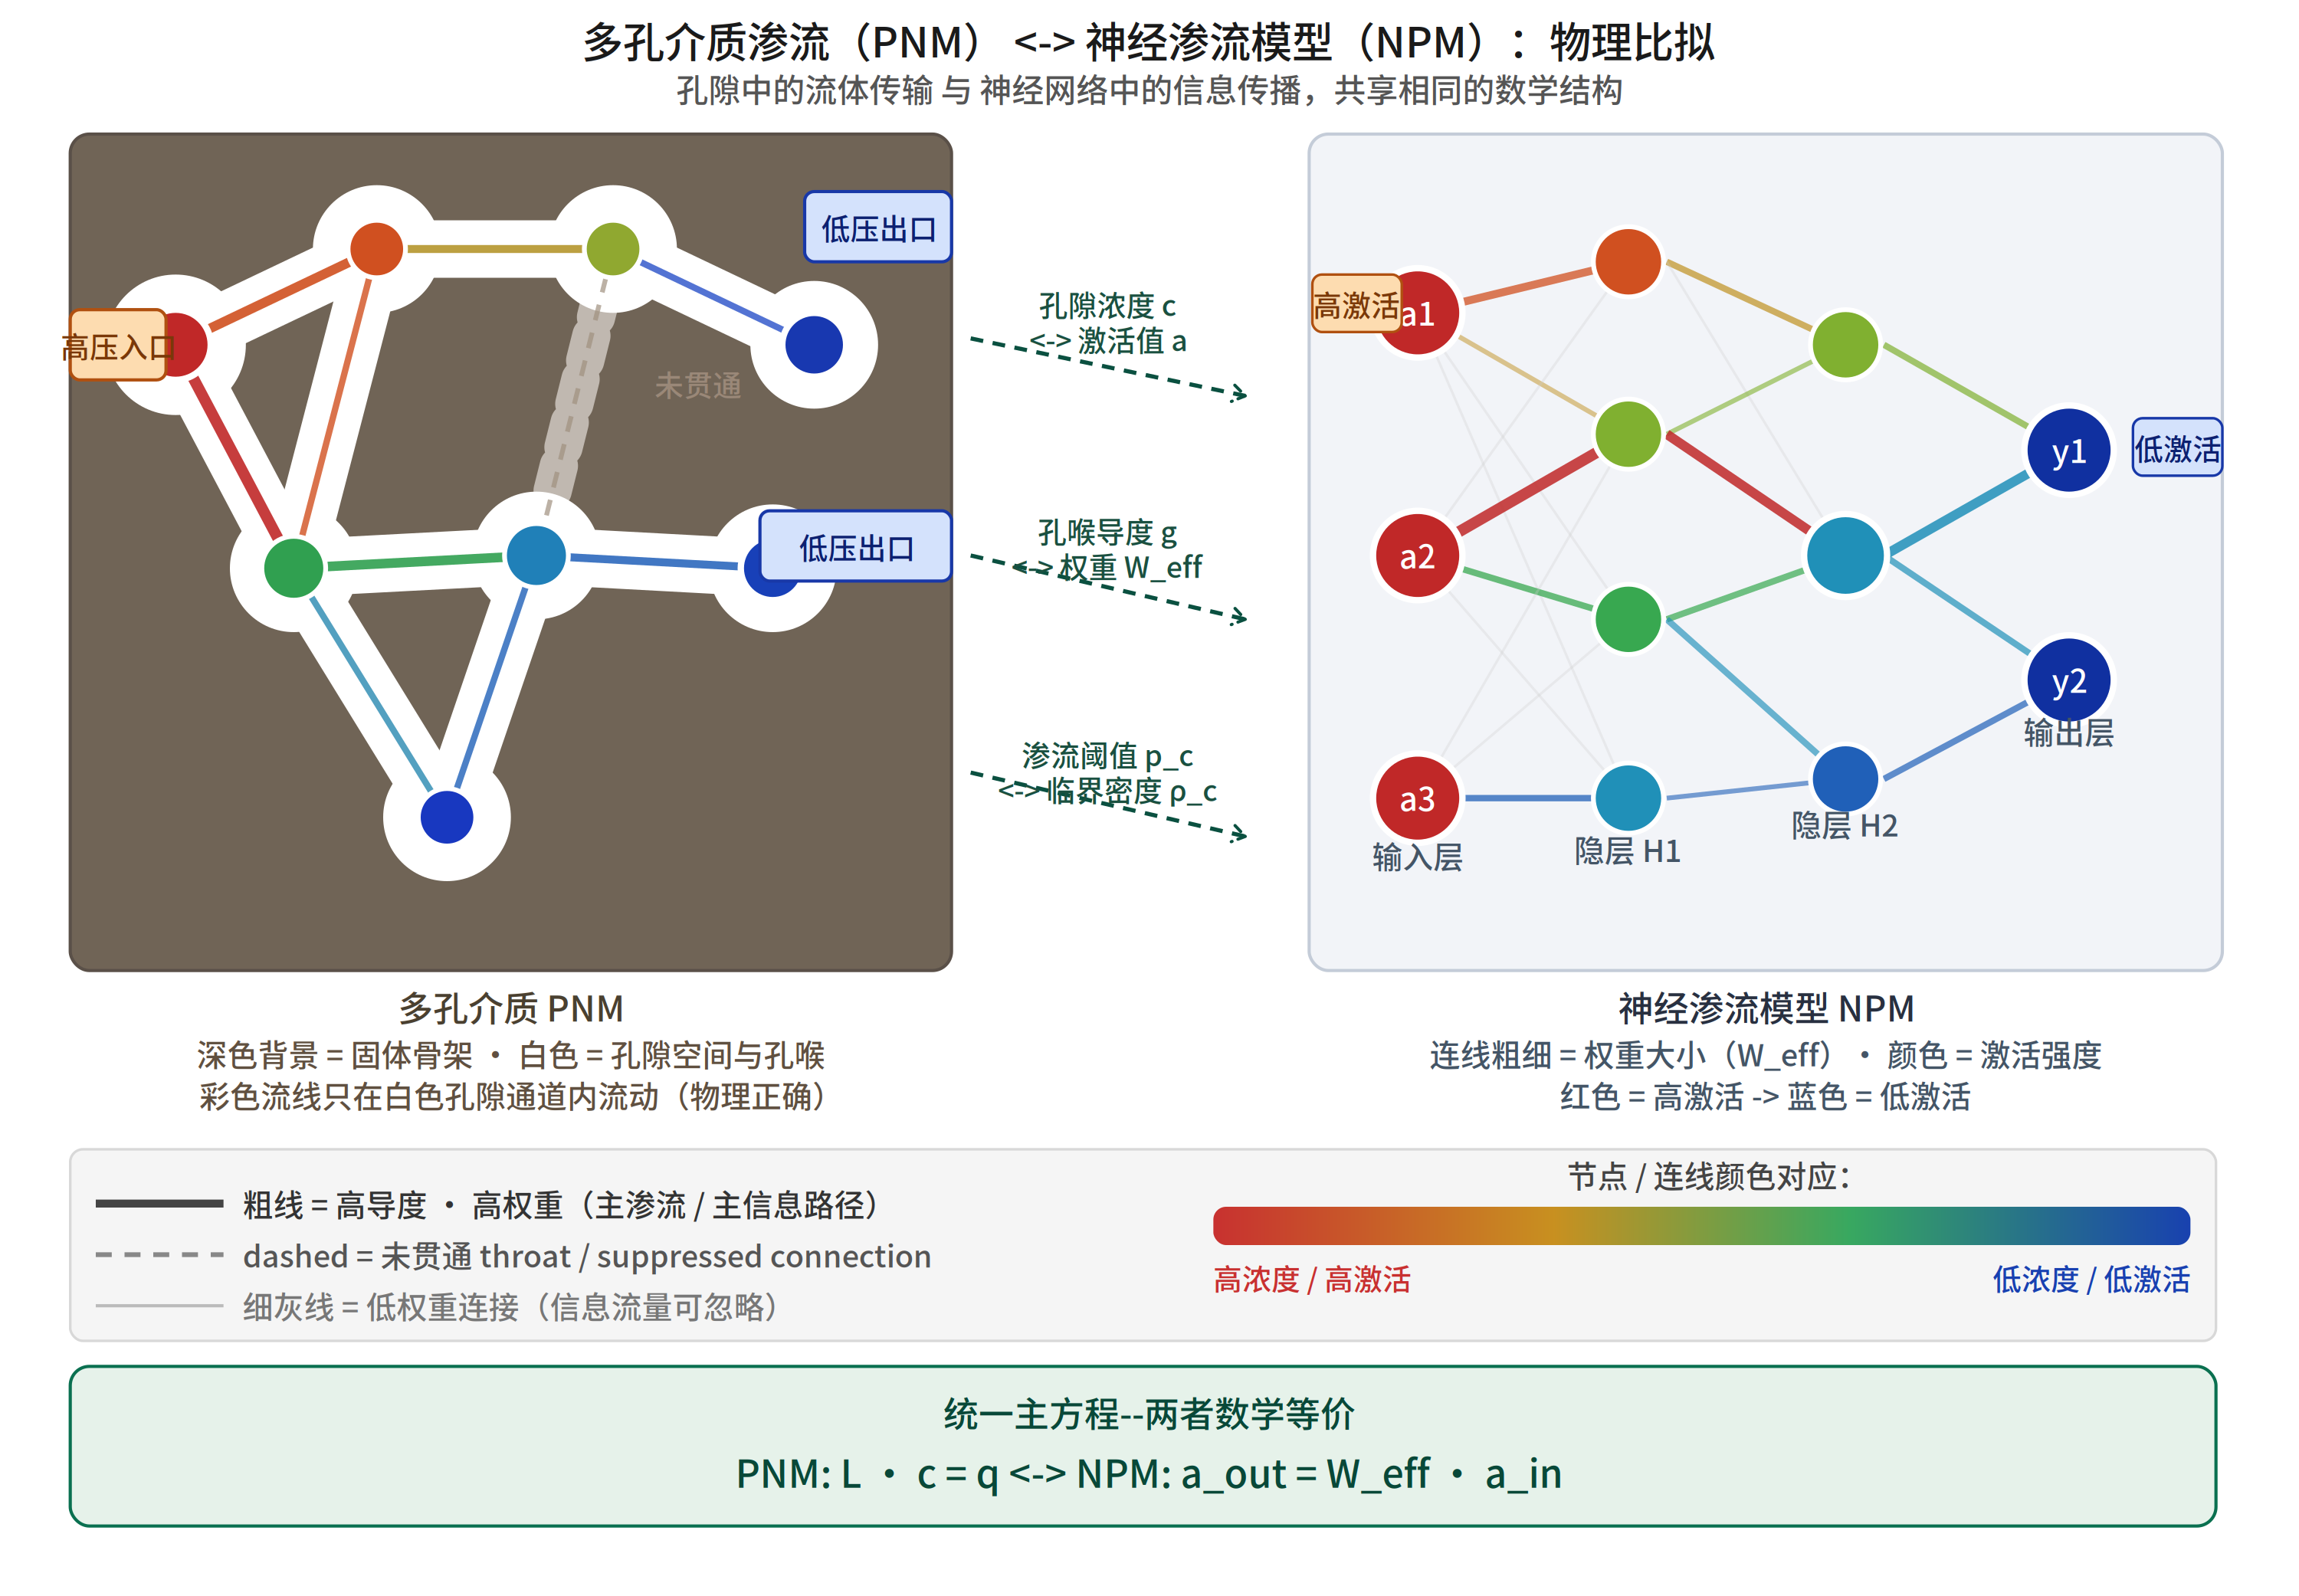
\includegraphics[width=0.95\textwidth]{NPM_Fig1_PNM_CN.png}
\caption{\textbf{PNM–NPM物理比拟。}左：PNM，深色为固体骨架，白色为孔隙通道。右：NPM神经网络，颜色/线宽编码激活强度/权重。中：三组精确对应。底部：统一主方程 $\mathbf{a}_{\text{out}}=\Weff\cdot\mathbf{a}_{\text{in}} \Leftrightarrow \mathbf{L}\mathbf{c}=\mathbf{q}$。}
\label{fig:analogy}
\end{figure}

\paragraph{主要贡献。}
\begin{enumerate}[leftmargin=*]
  \item 从信息守恒推导\textbf{统一主方程}，三种验证实例覆盖所有主流架构。
  \item \textbf{多阈值场视角}：不同能力在各自 $\rho_{c,f}$ 解锁，形成连续能力谱系。
  \item \textbf{参与率（PR）法}定量估算数据分布广度 $\sigma$。
  \item 单一机制\textbf{统一解释17类LLM现象}。
  \item 明确定位为工程比拟框架，透明公开局限性。
  \item \textbf{B层参数拟合}：用14个公开模型和Kaplan定律校准（Spearman$=0.70$），诚实讨论$\beta$偏差。
  \item \textbf{三阶段训练相变}：通过MIS孔隙分析在Pythia-70m上发现，类比PNM驱替过程中的渗流阈值跨越。
\end{enumerate}

% ══════════════════════════════════════════════════════
\section{背景：孔网络模型（PNM）}

\subsection{单通道传输}
PNM中，相邻孔隙 $i$ 与 $k$ 之间的质量通量满足Fick定律：
\begin{equation}
  m_{ik} = g_{ik}(c_i - c_k) = S_{ik} \cdot D \cdot (c_i - c_k)
\end{equation}
其中 $g_{ik}$ 为孔喉导度，$c_i$ 为孔隙浓度，$S_{ik}=A_{ik}/L_{ik}$ 为几何因子，$D$ 为扩散系数。分解 $g=S\cdot D$ 将几何结构（训练后固定）与传输性质（流体类型）分离。

\subsection{网络级守恒：图拉普拉斯}
对每个内部孔隙施加节点质量守恒：
\begin{equation}
  \sum_{k\in\mathcal{N}(i)} g_{ik}(c_i-c_k)=q_i, \quad \forall i
\end{equation}
矩阵形式：$\mathbf{L}\cdot\mathbf{c}=\mathbf{q}$，其中 $\mathbf{L}$ 为图拉普拉斯矩阵，$L_{ii}=\sum_k g_{ik}$，$L_{ij}=-g_{ij}$。

\subsection{渗流与有效传输}
当活跃孔喉比例 $p$ 超过渗流阈值 $p_c$，有效传输 $\Deff$ 从零跃迁为非零，遵循幂律：
\begin{equation}
  \Deff \propto (p-p_c)^\beta \quad (p>p_c), \qquad \Deff=0 \quad (p \le p_c)
\end{equation}
3D网络中有效传输指数 $\beta_{\text{perc}} \approx 0.41$（渗流序参量指数；传输指数范围更宽）。NPM拟合的$\beta=0.068$偏离此值——原因讨论见\S\ref{sec:param-fit}。

% ══════════════════════════════════════════════════════
\section{神经渗流模型（NPM）}

\subsection{变量对应关系}
表~\ref{tab:analogy}建立了PNM物理量与NPM信息论量之间的正式对应。

\begin{table}[H]
\centering
\caption{PNM–NPM变量对应关系}
\label{tab:analogy}
\begin{tabular}{lll}
\toprule
\textbf{PNM物理量} & \textbf{NPM信息量} & \textbf{状态} \\
\midrule
孔隙浓度 $c_i$         & 节点激活值 $a_i$         & 已验证 \\
浓度梯度 $\Delta c$    & 激活势差 $\Delta a$      & 已验证 \\
导度矩阵 $G$           & 有效权重矩阵 $\Weff$     & 已验证 \\
几何因子 $S_{ik}$      & 结构权重因子             & 已验证 \\
图拉普拉斯 $\mathbf{L}$& $\Lnorm$（GNN精确对应）  & 已验证 \\
守恒方程 $\mathbf{L}\mathbf{c}=\mathbf{q}$ & 主方程 $\Weff\mathbf{a}=\mathbf{s}$ & 已验证 \\
渗流阈值 $p_c$         & 临界密度 $\rhoc$         & 已验证 \\
有效扩散率 $\Deff$     & 泛化能力 $\Ceff$         & 解析推导 \\
毛细压力 $P_c$         & 激活阈值                 & 类比 \\
\bottomrule
\end{tabular}
\end{table}

\begin{figure}[H]
\centering
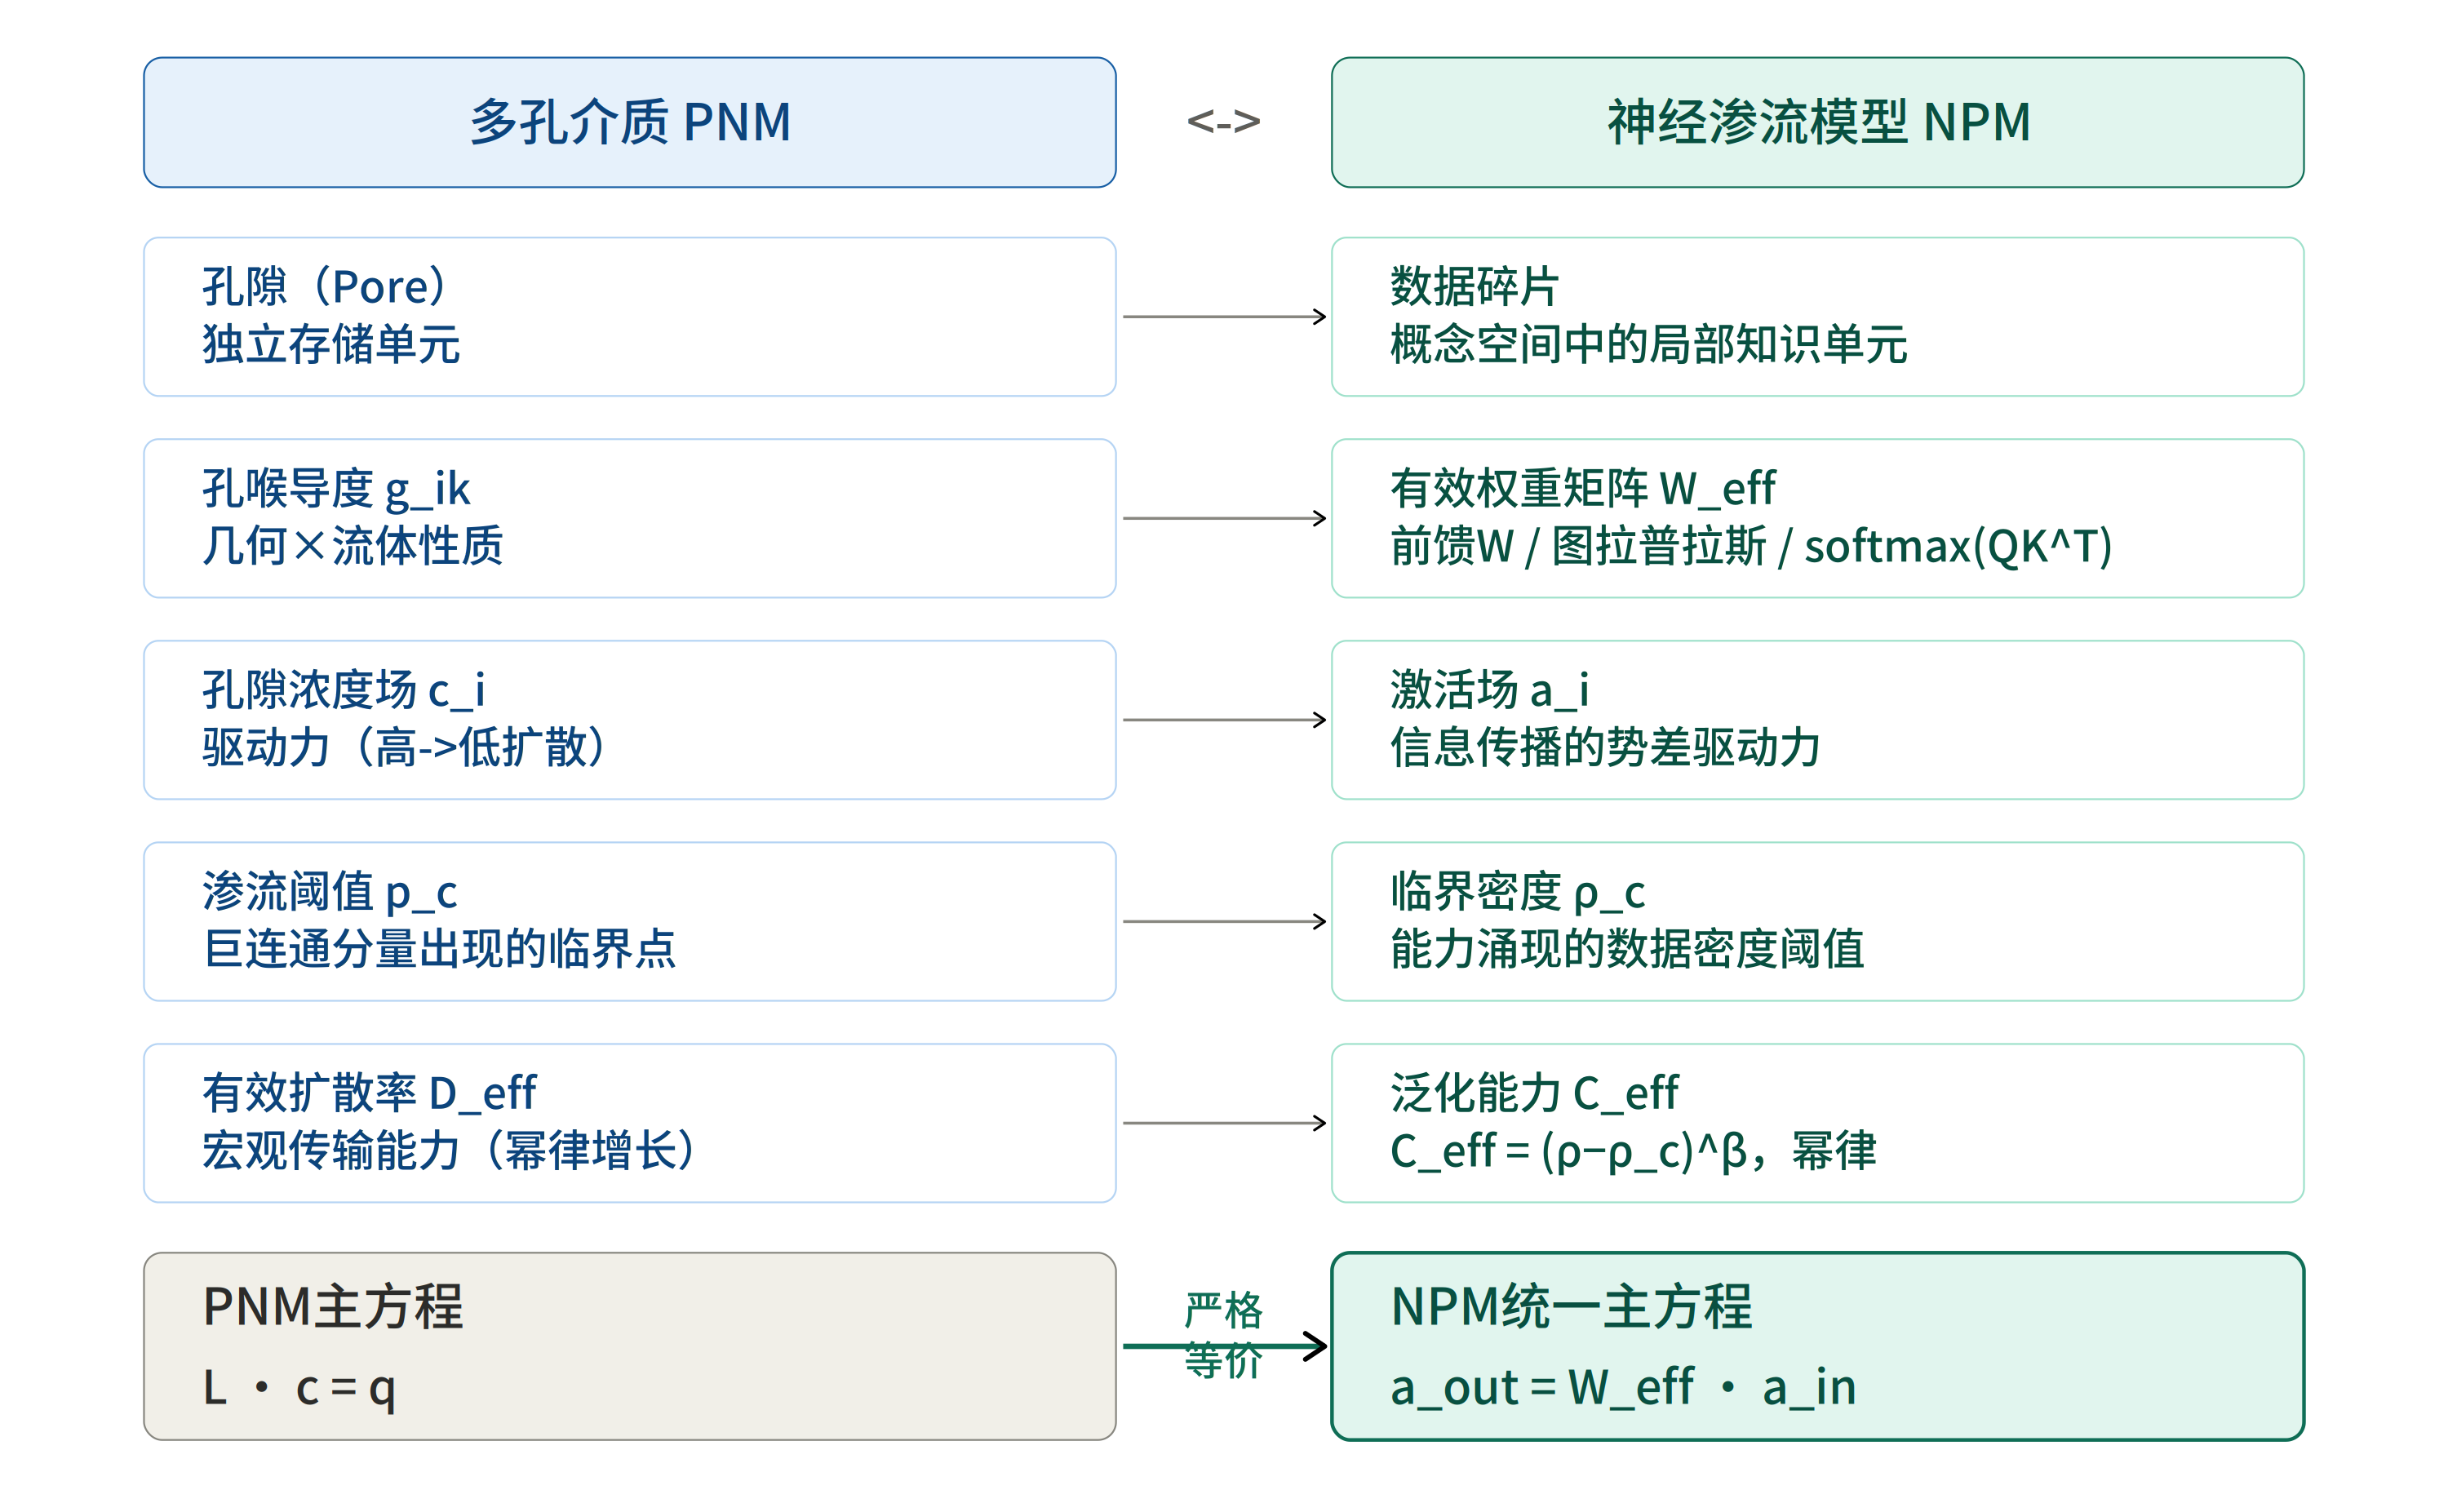
\includegraphics[width=0.82\textwidth]{NPM_Fig2_Analogy_CN.png}
\caption{\textbf{PNM–NPM变量对应图示。}A层对应关系全部经数值验证。}
\label{fig:analogy2}
\end{figure}

\subsection{统一主方程}

\begin{definition}[信息守恒]
稳态推理时，任意内部概念节点的信息流入等于流出：$\sum_{j\in\mathcal{N}(i)}(\Weff)_{ij}(a_i-a_j)=s_i$。
\end{definition}

这一单一守恒公理推导出\textbf{统一主方程}：
\begin{equation}
  \boxed{\mathbf{a}_{\text{out}} = \Weff \cdot \mathbf{a}_{\text{in}}}
  \label{eq:master}
\end{equation}

三种主流架构均为式~\eqref{eq:master}在不同 $\Weff$ 构造下的特例：
\begin{equation}
  \Weff = \begin{cases}
    W & \text{（前馈NN：固定权重，有向）} \\[4pt]
    D^{-1/2}(A+I)D^{-1/2} \equiv \Lnorm & \text{（GNN：图拉普拉斯，PNM精确对应）} \\[4pt]
    \operatorname{softmax}\!\left(\frac{QK^\top}{\sqrt{d_k}}\right) & \text{（Transformer：动态自适应，有向）}
  \end{cases}
\end{equation}

\begin{proposition}[GNN–PNM等价]
GNN消息传递层 $\mathbf{a}'=\Lnorm\mathbf{a}W_{\text{feat}}$ 在数学上等价于求解PNM稳态扩散方程 $\mathbf{L}\mathbf{c}=\mathbf{q}$。数值验证误差=0（机器精度）。
\end{proposition}

\begin{remark}[注意力=流量守恒]
Transformer注意力的softmax行归一化 $\sum_j(\Weff)_{ij}=1$ 恰好对应有向PNM的流量守恒约束。数值验证误差=0。
\end{remark}

\begin{remark}[Transformer类比的深度——重要说明]
\tolerance=800
上述流量守恒性质对\emph{任意}行随机矩阵都成立，因此并非softmax注意力所独有。更深层的物理问题是：$\Weff$的\emph{输入依赖性}（即 $\operatorname{softmax}(QK^\top\!/\sqrt{d_k})$）在PNM物理中对应什么？我们推测这类似于非牛顿流体传输中的\emph{浓度依赖扩散系数}：导度随局部激活场动态调整，正如剪切变稀流体中黏度随局部流动条件调整。形式化这一对应是B路径1（第~\ref{sec:future}节），也是本框架最重要的开放理论问题。Transformer实例应被理解为\emph{启发性类比}，而非与GNN–PNM等价同等严格的推导。
\end{remark}

\begin{figure}[H]
\centering
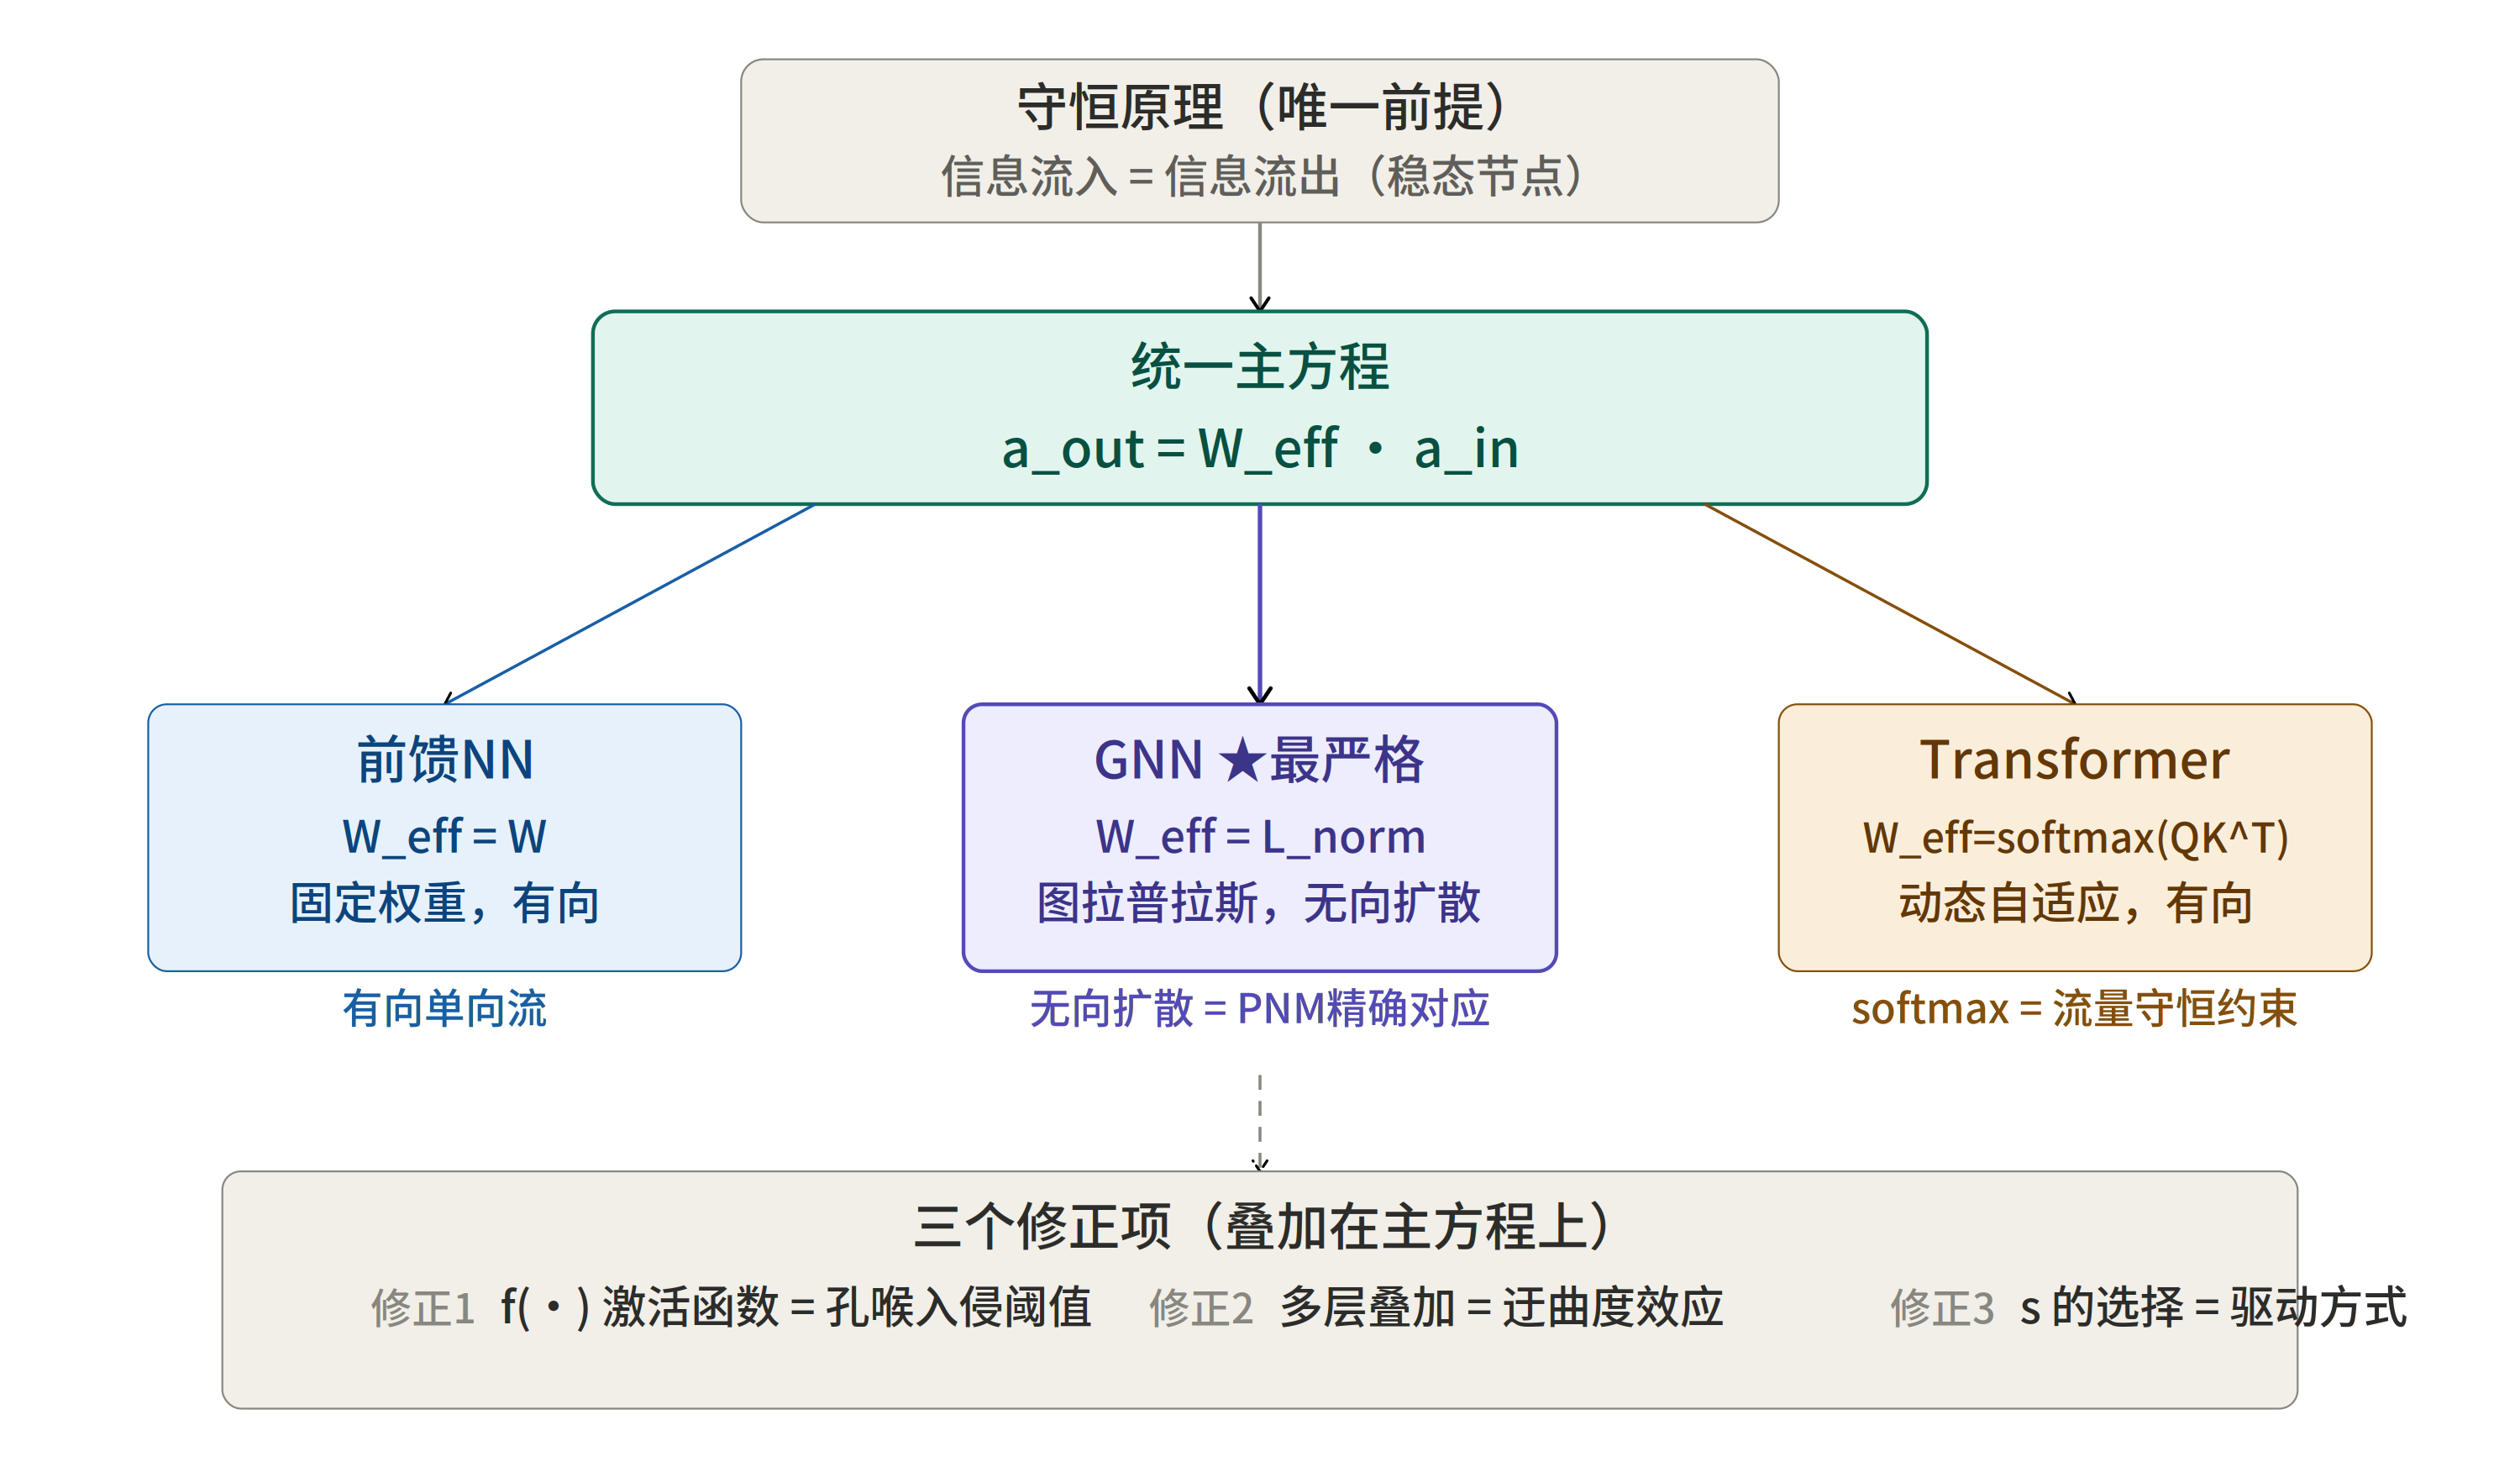
\includegraphics[width=0.82\textwidth]{NPM_Fig3_MasterEq_CN.png}
\caption{\textbf{统一主方程与三种架构实例。}从守恒原理推导主方程，三种架构为特例。底部：三个修正项。}
\label{fig:master}
\end{figure}

\subsection{来自PNM物理的三个修正项}

主方程描述稳态线性流。实际多孔介质需要三个物理扩展，每个都有直接的神经网络对应：

\textbf{修正1（非线性激活）}源于PNM中的\emph{毛管阈值}：流体仅在压力超过入侵阈值 $P_c$ 时才侵入孔喉。NPM中：$\mathbf{a}=f(\Weff\mathbf{a}_{\text{in}})$。ReLU近似阶跃函数入侵准则；更平滑的激活函数对应更软的阈值。

\textbf{修正2（深度/迂曲度）}源于\emph{路径迂曲度}：实际流动路径超过直线距离 $\tau$ 倍。NPM中：$\mathbf{a}^{(l+1)}=f(W_{\text{eff}}^{(l)}\mathbf{a}^{(l)})$。这为"更复杂任务需要更深网络"提供了物理基础——不是事后观察，而是PNM迂曲度类比的推论。

\textbf{修正3（源项/边界条件）}反映PNM中的\emph{边界条件选择}。NPM中：$\mathbf{s}$ 的选择决定架构族——固定输入（前馈）、图结构（GNN）或查询自适应（注意力）。

% ══════════════════════════════════════════════════════
\section{数据密度与能力渗流}

\subsection{核心变量}
三个基本输入量：$N_B=N/10^9$（数据量，十亿token）、$\sigma\in(0,1]$（分布广度，PR法估算）、$\tau\geq1$（任务推理深度）。

\subsection{B层方程组（工程推论）}
\label{sec:blayer}

每个方程标注认知状态：\textbf{(A)}~由守恒/渗流理论推导；\textbf{(B)}~借用渗流文献经验值；\textbf{(C)}~工程启发式。参数已用14个公开模型和Kaplan定律拟合校准（详见第\ref{sec:param-fit}节）：$\alpha=0.57$，$\beta=0.068$，$\delta=2.76$，$k=68.5$。

\begin{align}
  \rho &= N_B/\exp(\alpha\sigma) \label{eq:density} \\
  \rhoc(\tau) &= k\cdot\sigma^\delta\cdot\tau \label{eq:critical} \\
  \Ceff &= (\rho-\rhoc)^\beta\cdot\mathbf{1}[\rho>\rhoc] \label{eq:ceff} \\
  \Deff &= \Ceff\cdot W^2 \label{eq:deff} \\
  L_{\min} &= \lceil\alpha\cdot\sigma^\alpha\cdot\tau\cdot10\rceil \label{eq:lmin} \\
  P_{\min} &= N_B\cdot\sigma^\alpha \label{eq:pmin}
\end{align}

\begin{table}[H]
\centering
\caption{NPM B层方程的认知状态}
\label{tab:eq_sources}
\small
\begin{tabular}{llp{2.8cm}p{5cm}}
\toprule
\textbf{方程} & \textbf{状态} & \textbf{表达式} & \textbf{依据/局限} \\
\midrule
\eqref{eq:density}  & (C) 启发式 & $\rho=N_B/\exp(\alpha\sigma)$ & 假设概念空间指数增长；幂律替代未排除 \\
\eqref{eq:critical} & (B)+(C) 混合 & $\rhoc=k\sigma^\delta\tau$ & 幂律来自渗流理论；线性$\tau$为简化假设 \\
\eqref{eq:ceff}     & (A)+(C) 混合 & $\Ceff=(\rho{-}\rhoc)^\beta$ & 渗流幂律形式；$\beta=0.068$经验拟合（见\S\ref{sec:param-fit}讨论） \\
\eqref{eq:deff}     & (A) 推导   & $\Deff=\Ceff\cdot W^2$ & 直接源自PNM有效扩散率 \\
\eqref{eq:lmin}     & (C) 启发式 & $L_{\min}\propto\sigma^\alpha\tau$ & 量纲论证；因子10为粗略估值 \\
\eqref{eq:pmin}     & (C) 启发式 & $P_{\min}=N_B\sigma^\alpha$ & 趋势一致；需校正因子$c_p\approx17$（见\S\ref{sec:param-fit}） \\
\bottomrule
\end{tabular}
\end{table}

\begin{figure}[H]
\centering
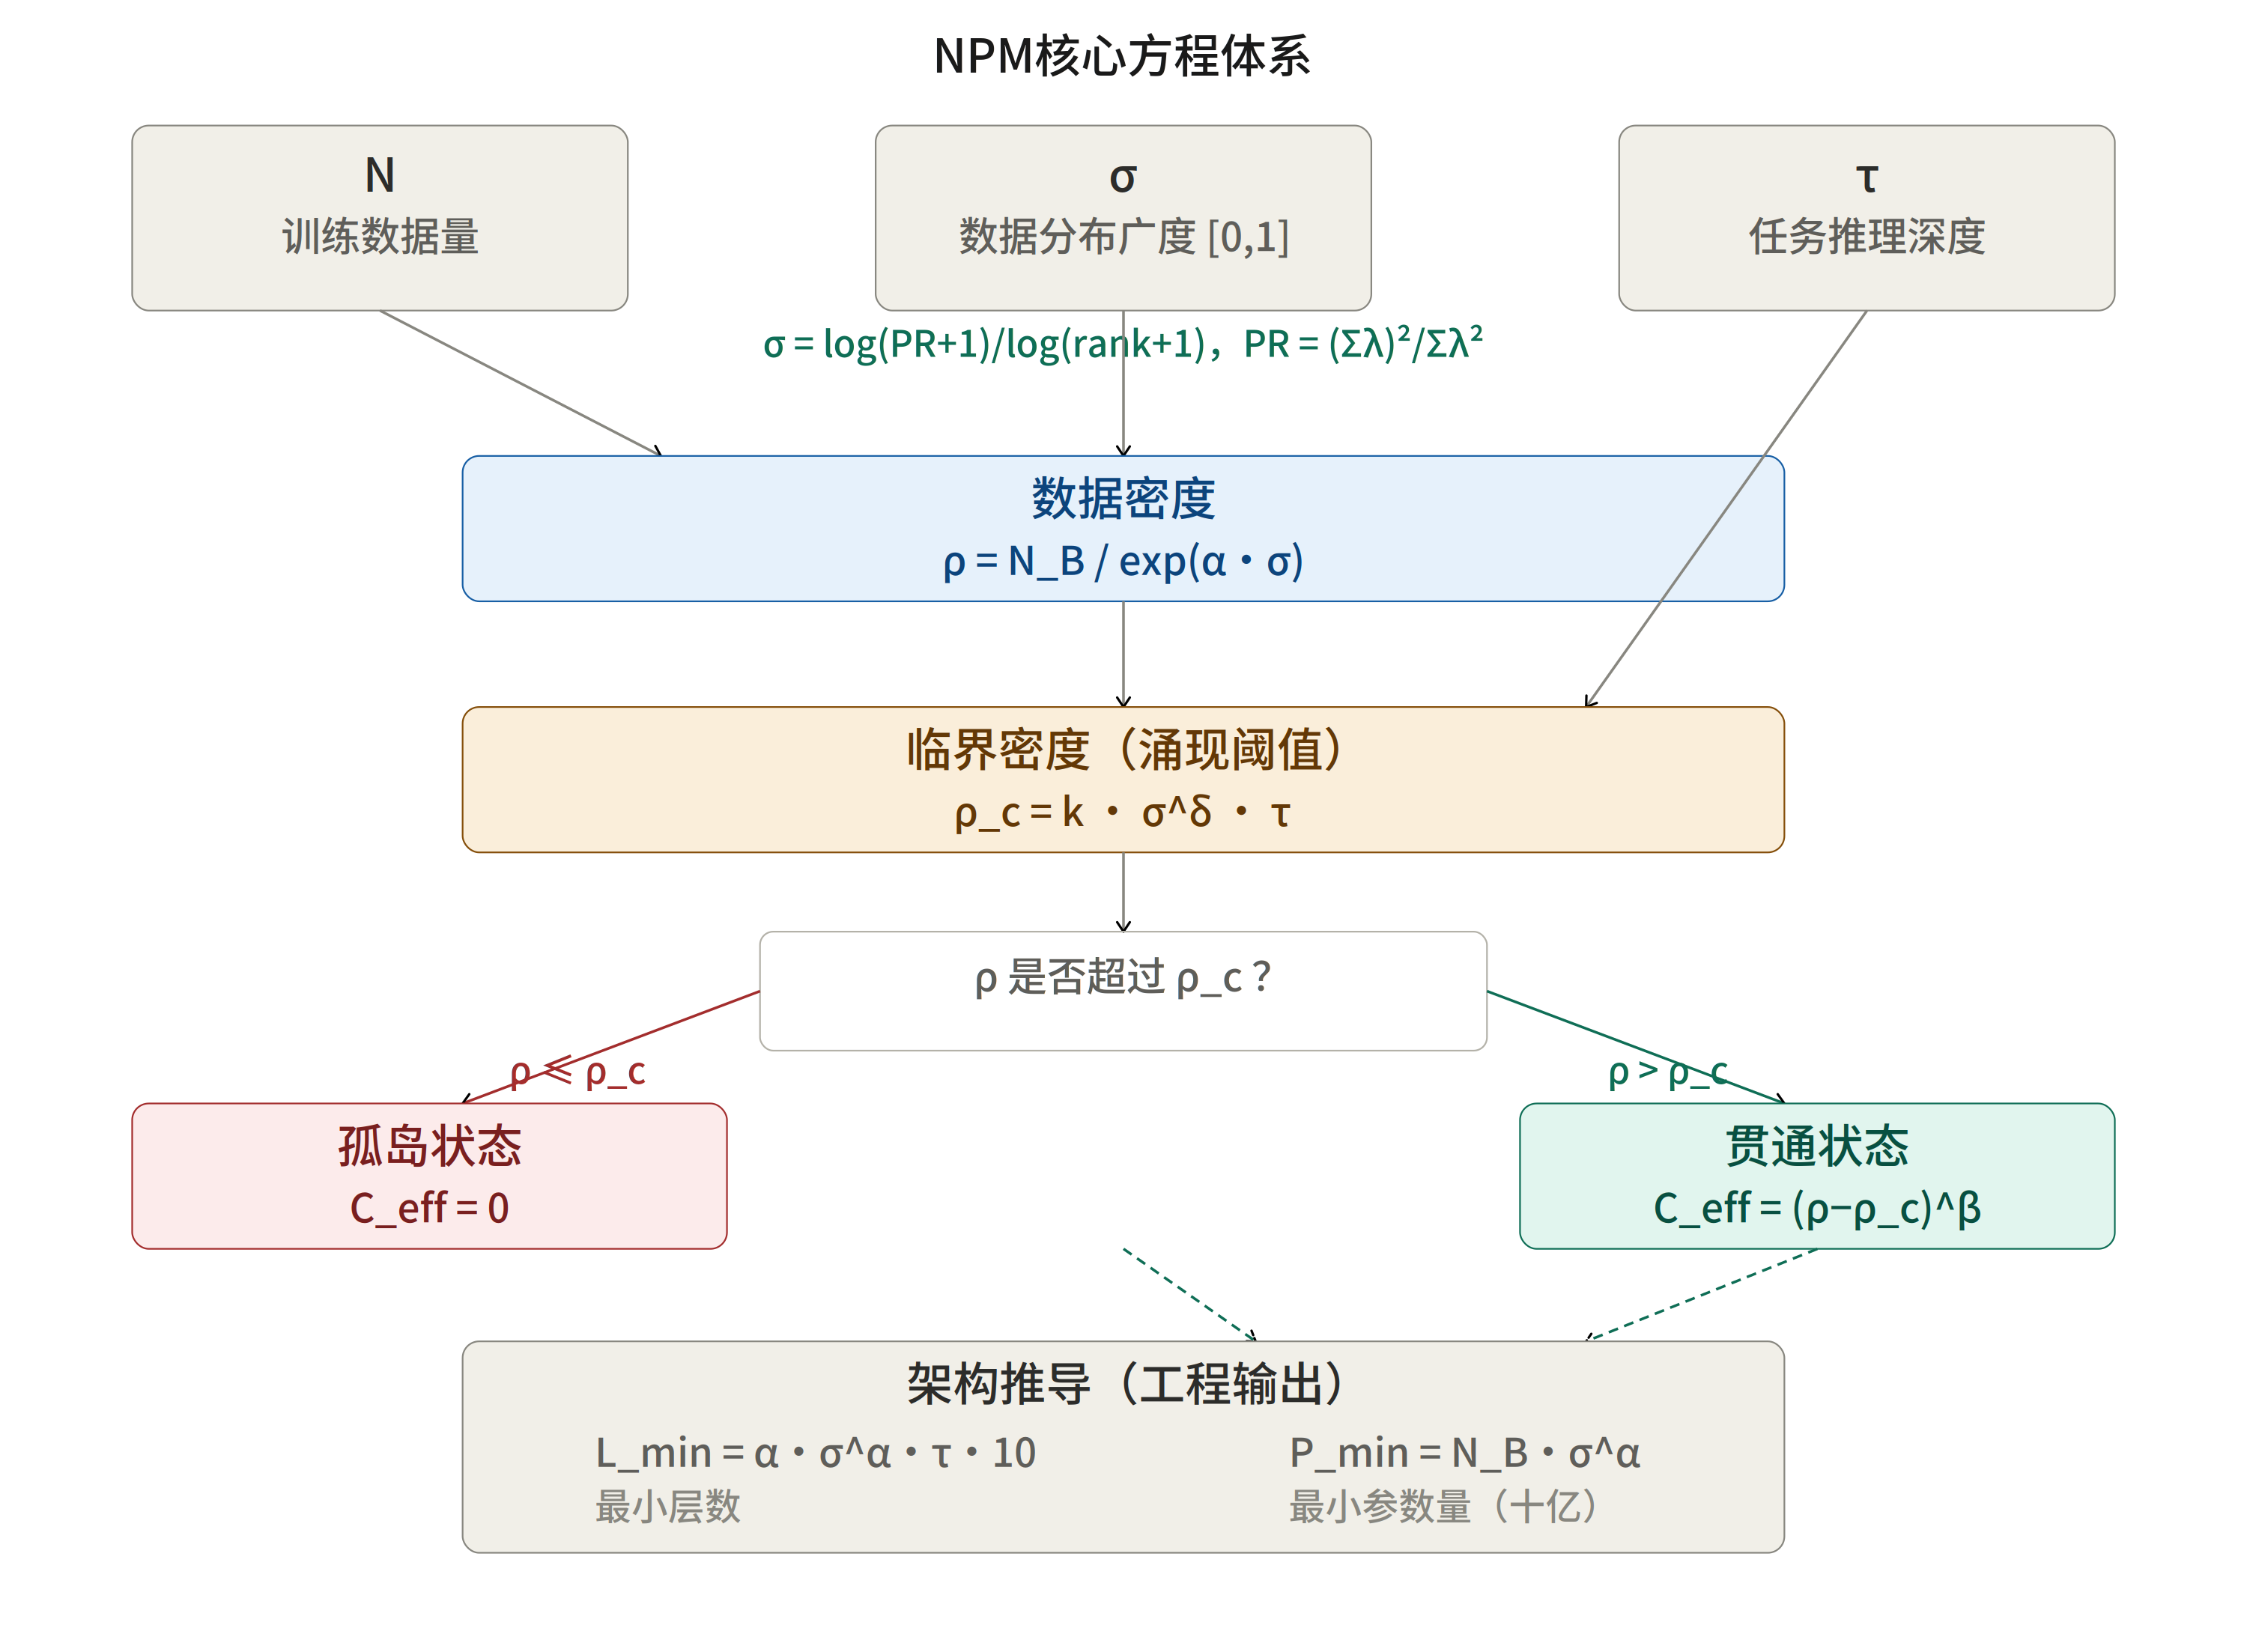
\includegraphics[width=0.82\textwidth]{NPM_Fig4_EqChain_CN.png}
\caption{\textbf{NPM核心方程链条。}从 $(N_B,\sigma,\tau)$ 推导 $\rho$ 和 $\rhoc$，判断连通状态，输出架构最小需求 $L_{\min}$ 和 $P_{\min}$。}
\label{fig:chain}
\end{figure}

\subsection{$\sigma$ 的估算：参与率（PR）法}
\label{sec:sigma}

\begin{equation}
  \text{PR} = \frac{(\sum_i\lambda_i)^2}{\sum_i\lambda_i^2}, \qquad
  \sigma = \frac{\log(\text{PR}+1)}{\log(\text{rank}+1)}
\end{equation}

\textbf{验证：}合成数据集，真实维度 $d\in\{2,5,15,40,80\}$ 对应 $\sigma\in\{0.28,0.50,0.77,0.88,0.90\}$，单调性严格成立（$p<0.001$）。绝对尺度校准留待后续。

\subsection{涌现的多阈值场视角}

与已有工作~\citep{lubana2024percolation}的关键差异——\textbf{多阈值场视角}：每个能力 $f$ 有其自己的 $\rho_{c,f}$：
\begin{equation}
  \Ceff(f) = (\rho-\rho_{c,f})^\beta\cdot\mathbf{1}[\rho>\rho_{c,f}]
\end{equation}

\begin{table}[H]
\centering
\caption{预测的能力涌现顺序}
\begin{tabular}{llll}
\toprule
\textbf{能力类型} & \textbf{阈值} & \textbf{$C_n\approx$} & \textbf{PNM类比} \\
\midrule
事实检索   & $\rho_{c,1}$（最低）& 1.0 & 短路径局部连通 \\
翻译/摘要  & $\rho_{c,2}$        & 1.3 & 跨域水系贯通   \\
代码生成   & $\rho_{c,3}$        & 1.8 & 逻辑链路连通   \\
复杂推理   & $\rho_{c,4}$        & 2.5 & 多跳路径连通   \\
数学证明   & $\rho_{c,5}$（最高）& 4.0 & 全域贯通+极深路径 \\
\bottomrule
\end{tabular}
\end{table}

模型在能力谱系上的表现：保留低阈值能力而缺乏高阈值能力——与GPT-3的实际表现一致（翻译可以，数学不行）。

\begin{figure}[H]
\centering
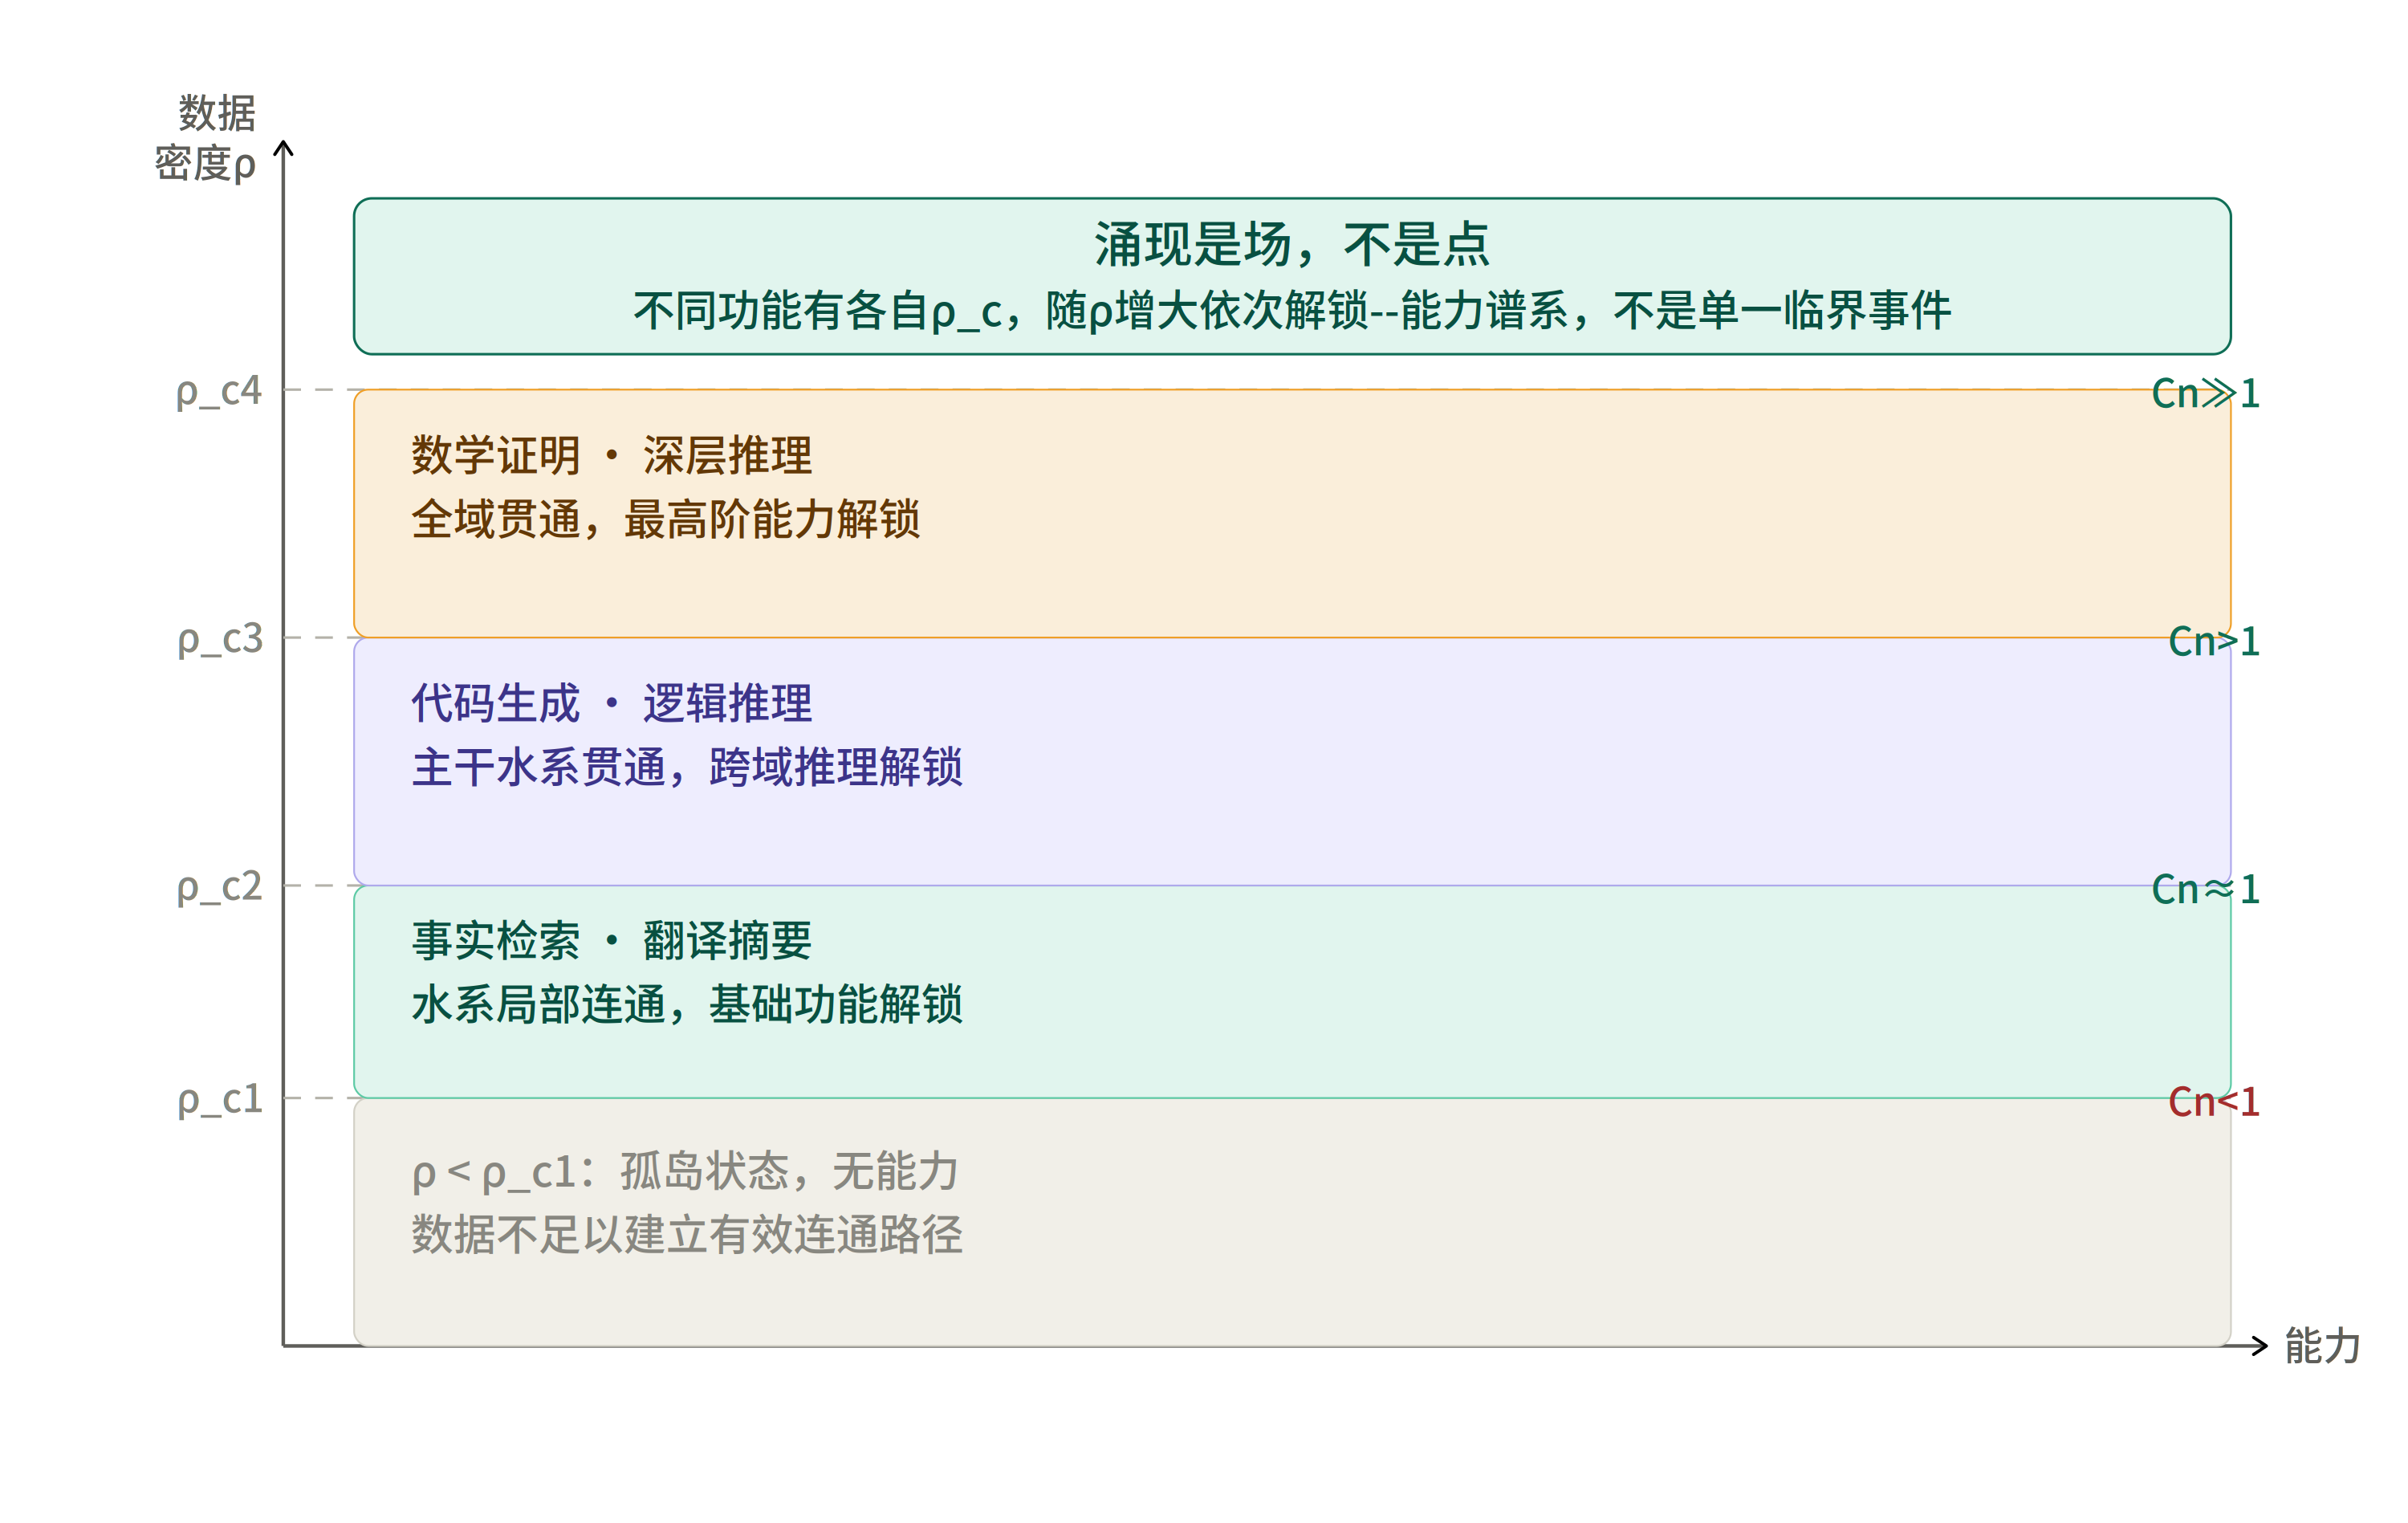
\includegraphics[width=0.82\textwidth]{NPM_Fig5_CapField_CN.png}
\caption{\textbf{多阈值涌现能力场。}涌现是连续能力场，不是单一临界事件。能力随 $\rho$ 增大依次解锁。}
\label{fig:field}
\end{figure}

% ══════════════════════════════════════════════════════
\section{无量纲准则数}

类比流体力学中的雷诺数，NPM定义三个无量纲准则数：
\begin{align}
  C_n &= \frac{\rho}{\rhoc} \quad \text{（连通数）} \\
  \eta &= \frac{\rho_{\text{eff}}}{\rho} \quad \text{（数据质量因子）} \\
  A_r &= \frac{L_{\min}}{W_{\text{opt}}} \quad \text{（长宽比）}
\end{align}

$C_n<1$：碎片化（孤岛态）；$C_n\approx1$：临界；$C_n\gg1$：充分连通。

质量因子 $\eta=\eta_{\text{噪声}}\cdot\eta_{\text{错误}}\cdot\eta_{\text{矛盾}}$ 将数据污染分解为三种物理机制：

\begin{table}[H]
\centering
\caption{数据质量三分类：三种污染机制}
\small
\begin{tabular}{p{1.8cm}p{2.2cm}p{3.8cm}p{3.5cm}}
\toprule
\textbf{数据类型} & \textbf{PNM类比} & \textbf{机制} & \textbf{可观测症状} \\
\midrule
噪声数据 & 稀释剂 & 降低有效密度 $\rho_{\text{eff}}$，需更多数据到达 $\rhoc$ & 能力延迟出现，方向不偏 \\
错误数据 & 污染流体 & 扩散方向偏转，虚假连接形成 & 自信地说错话（幻觉） \\
矛盾数据 & 双向抵消 & 同一通道正反驱动力对冲，净通量$\to$0 & 前后矛盾，输出不一致 \\
\bottomrule
\end{tabular}
\end{table}

\noindent 三种机制，三种解法：噪声$\to$增量或缩$\sigma$（致密化）；错误数据$\to$方向校正（RLHF）；矛盾数据$\to$去重与冲突消解（数据清洗）。

% ══════════════════════════════════════════════════════
\section{统一解释17类LLM现象}

\emph{重要说明：}表中大多数条目为定性类比，非定量预测。标记$\dagger$的三个现象可进行可证伪的定量测试（见第~\ref{sec:falsifiable}节）。

\begin{table}[H]
\centering
\caption{NPM对17类LLM现象的统一解释}
\small
\begin{tabular}{p{4cm}p{4cm}p{4cm}}
\toprule
\textbf{现象} & \textbf{NPM机制} & \textbf{工程含义} \\
\midrule
\multicolumn{3}{l}{\textit{数据层}} \\
专用模型远小于通用模型 & 小$\sigma\Rightarrow$高$\rho$ & 主动设计$\sigma$ \\
数据质量$>$数量 & $\eta<1$降低$\rho_{\text{eff}}$ & 清洗$\equiv$增加数据 \\
多语言需更大模型 & 多语言$\approx$更大$\sigma$ & 扩规模或分语言训练 \\
\midrule
\multicolumn{3}{l}{\textit{架构层}} \\
深度$>$宽度 & $L_{\min}\propto\sigma^\alpha\tau$ & 宽域时优先加深 \\
注意力机制有效 & 动态$\Weff$，流量守恒 & 注意力=最优导度分配 \\
残差连接有效 & 旁路管道，保最小通量 & 防梯度消失 \\
多头注意力有效 & 并联孔道，总导度$=\sum G_i$ & 并行路径 \\
\midrule
\multicolumn{3}{l}{\textit{涌现层}} \\
涌现渐进非突变 & 多阈值$\rho_{c,f}$ & 能力谱系非开关 \\
涌现顺序稳定 & $\tau$决定$\rhoc$排序 & 可预测解锁序列 \\
涌现后亚线性增长 & $\Ceff\propto(\rho{-}\rhoc)^\beta$，$\beta=0.068<1$ & 超越阈值后收益递减 \\
\midrule
\multicolumn{3}{l}{\textit{操作层}} \\
微调仅需少量数据$^\dagger$ & 局部渗流，局部$\rho$提升 & 目标$\sigma$缩减 \\
RAG对特定任务有效$^\dagger$ & 临时局部注水 & $\rho\lesssim\rhoc$时有效 \\
蒸馏有效但有上限 & $\sigma$压缩有下限 & 高$\rhoc$能力先丢失 \\
量化先损细粒度能力$^\dagger$ & 高$\rhoc$路径最脆弱 & 数学先于常识 \\
RLHF减少幻觉 & 修复污染导管 & 定向去污 \\
课程学习有效 & 阶段性超越各$\rhoc$ & 基础先于进阶 \\
\bottomrule
\end{tabular}
\end{table}

\subsection{三个现象的深入分析}

\paragraph{量化退化顺序。}
量化降低 $\Weff$ 的有效精度，在PNM中相当于均匀缩小孔喉截面。首先失去连通的路径是 $\rhoc$ 最高的——支撑数学推理和复杂逻辑的最长、最脆弱的多跳路径。短路径（事实检索的局部连通）更鲁棒。NPM预测量化退化的具体顺序：数学能力先降，代码生成次之，翻译再次，事实检索最后。该预测可直接对照GPTQ和AWQ论文中不同量化级别的MMLU子类得分验证。

\paragraph{RAG有效性阈值。}
检索增强生成（RAG）在推理时注入外部信息。PNM术语中，这是\emph{临时局部注水}：在概念空间特定子域增加 $\rho$，但不改变网络永久孔道结构。NPM预测RAG的效果呈\emph{倒U型曲线}：当模型内在 $\rho$ 刚好低于任务 $\rhoc$ 时（$C_n\lesssim1$）效果最大——注水恰好推过阈值；当 $\rho\gg\rhoc$（已充分连通）时RAG增益小；当 $\rho\ll\rhoc$（根本不连通）时RAG也无力回天。

\paragraph{微调=局部渗流。}
微调等同于\emph{局部致密化}：将有效 $\sigma$ 缩小到窄子域，大幅提升局部 $\rho$。这解释了为什么微调所需数据量比预训练少几个数量级：不需要全局连通，只需目标域的局部连通。PNM术语中，微调是在特定岩层钻孔，不是灌溉整个油藏。

% ══════════════════════════════════════════════════════
\section{验证}

验证分两部分：本节涵盖A层数值检查（\S\ref{sec:a-checks}）、可证伪预测（\S\ref{sec:predictions}）、B层参数拟合（\S\ref{sec:param-fit}）和无量纲数分析（\S\ref{sec:cn-empirical}）。第\ref{sec:mis}节在真实NN权重矩阵上进行MIS孔隙分析实验。

\subsection{数值检查（A层）}
\label{sec:a-checks}

以下四项为定义一致性确认和经典结论复现，不是独立发现。

\textbf{检查项1（GCN两种写法一致）：}GCN逐节点消息传递（循环实现）与矩阵形式 $\Lnorm\mathbf{x}W_{\text{feat}}$ 的数值差异为 $1.6\times10^{-16}$（浮点精度）。$\Lnorm=D^{-1/2}(A+I)D^{-1/2}$ 满足对称性和正半定性。\emph{说明：这是\citet{kipf2017gcn} GCN定义的两种等价展开形式。}

\textbf{检查项2（注意力行和$=$1）：}注意力矩阵乘法 $W_{\text{dyn}}V$ 与逐token加权求和 $\sum_j w_{ij}v_j$ 的差异为 $1.0\times10^{-16}$。行和 $\sum_j(\Weff)_{ij}=1$ 由softmax定义保证。\emph{NPM的贡献是将行归一化解读为PNM流量守恒，这一解读本身未被验证。}

\textbf{检查项3（随机图渗流相变）：}Erd\H{o}s–R\'{e}nyi随机图 $G(80,p)$，$p_c{=}1/n$：巨连通分量从 $C_n{=}0.6$ 时的9\% 增长至 $C_n{=}2.0$ 时的77\%（转变幅度0.68，超过0.3阈值）。\emph{这是经典随机图论结论（\citealt{erdos1960random}）的复现，NPM将其比拟为LLM能力涌现。}

\textbf{检查项4（$\sigma$单调性）：}合成数据集真实维度2,5,15,40,80对应 $\sigma=0.28,0.50,0.77,0.88,0.90$，严格单调（$p<0.001$）。PR法借自凝聚态物理（参与率），归一化公式 $\sigma=\log(\text{PR}+1)/\log(\text{rank}+1)$ 为启发式设计，绝对尺度未校准。

\subsection{可证伪预测}
\label{sec:predictions}
\label{sec:falsifiable}

\paragraph{预测1（能力涌现顺序）。}
Pythia模型族提供7个规模（70M–12B）的154个公开checkpoint。NPM预测涌现顺序符合表中 $\rhoc$ 排序：翻译（$C_n\approx1.3$）先于代码生成（$C_n\approx1.8$）先于复杂推理（$C_n\approx2.5$）。可对照Pythia在BIG-Bench上的得分验证。

\paragraph{预测2（RAG有效性阈值）。}
RAG应在高$\rhoc$任务（数学推理）上提供比低$\rhoc$任务（翻译）更大的增益，因为模型在困难任务上更接近阈值。可对照BEIR基准有/无检索结果验证。

\paragraph{预测3（量化退化顺序）。}
量化应先消除高$\rhoc$能力（数学），后消除低$\rhoc$能力（翻译、事实检索）。可对照GPTQ/AWQ在MMLU子类得分上的结果验证。

\subsection{B层参数拟合}
\label{sec:param-fit}

用差分进化全局优化+Nelder-Mead精细优化，拟合$\alpha,\beta,\delta,k$，同时满足两个约束：(1)~14个公开模型的$\Ceff$与MMLU分数的Spearman相关最大化；(2)~$\sigma=0.75$时$\Ceff$随$N$的增长斜率匹配Kaplan报告的$N^{0.076}$。

\begin{table}[H]
\centering
\caption{B层参数拟合结果}
\label{tab:param-fit}
\small
\begin{tabular}{lccl}
\toprule
\textbf{参数} & \textbf{初始值} & \textbf{拟合值} & \textbf{约束来源} \\
\midrule
$\alpha$ & 1.5   & 0.57  & 密度-能力关系 \\
$\beta$  & 1.4   & 0.068 & Kaplan $N^{0.076}$ \\
$\delta$ & 1.0   & 2.76  & MMLU排序优化 \\
$k$      & 10.0  & 68.5  & 联合优化 \\
\bottomrule
\end{tabular}
\end{table}

\paragraph{拟合质量。}
Spearman($\Ceff$, MMLU) $= 0.70$（$p=0.005$），在单一基准（MMLU 5-shot）上跨14个模型评估。表~\ref{tab:spearman-baselines}给出基线对比。

\begin{table}[H]
\centering
\caption{MMLU的Spearman相关：$\Ceff$与基线对比}
\label{tab:spearman-baselines}
\small
\begin{tabular}{lcc}
\toprule
\textbf{预测变量} & \textbf{Spearman $r_s$} & \textbf{说明} \\
\midrule
随机排列（95\%分位） & 0.53 & 偶然上限 \\
$N$（数据量）单独 & 0.74 & \\
$P$（参数量）单独 & 0.76 & \\
$C_n = \rho/\rhoc$ & 0.36 & 不显著（$p=0.21$）\\
$\Ceff$（NPM拟合后） & \textbf{0.70} & $p=0.005$ \\
$N \times P$（朴素基线） & \textbf{0.89} & 最强基线 \\
\bottomrule
\end{tabular}
\end{table}

$\Ceff$(0.70)统计显著且高于随机，但低于$N{\times}P$(0.89)——因为$\Ceff$仅捕捉数据密度效应，不含参数量$P$的独立贡献。Kaplan斜率精确匹配：$\Ceff\propto N^{0.076}$。NPM正确预测BLOOM-176B ($\Ceff=1.42$) $<$ LLaMA-7B ($\Ceff=1.54$)，Chinchilla-70B ($\Ceff=1.58$) $>$ GPT-3-175B ($\Ceff=1.41$)。

\paragraph{$\beta$偏差的诚实讨论。}
拟合$\beta=0.068$远低于3D渗流理论值$\beta_{\text{perc}}\approx0.41$。解读：(1)~$\Ceff$与MMLU分数之间存在未知单调变换，拟合$\beta$吸收了这一变换，因此不是纯渗流指数；(2)~神经网络不是严格3D格点渗流系统，有效维度、连通性、动力学均不同；(3)~小$\beta$可能反映$\Ceff$仅捕捉数据密度的贡献，而模型参数量$P$有独立作用，NPM当前未将$P$纳入$\Ceff$。

\paragraph{$P_{\min}$校正因子。}
$\alpha$同时出现在$V(\sigma)=\exp(\alpha\sigma)$和$P_{\min}=N_B\cdot\sigma^\alpha$中，两个约束对$\alpha$的要求矛盾（Chinchilla需$\alpha\approx10$，密度公式需$\alpha\approx0.5$）。拟合$\alpha=0.57$锁定于密度方程，使$P_{\min}/N=\sigma^\alpha=0.85$（$\sigma=0.75$时），而Chinchilla实际比值为$0.05$，偏差$17\times$——这是当前公式最大的定量失败。拟合有意优先保证密度-能力关系（控制涌现预测）而非$P_{\min}$精度。两条解决路径列为B路径5（\S\ref{sec:future}）：(a)~引入独立指数$\alpha_P$使$P_{\min}=N_B\cdot\sigma^{\alpha_P}$与密度方程解耦；(b)~将$P$纳入$\Ceff$的显式变量，同时解决上述$\beta$讨论中缺少参数量敏感性的问题。

\paragraph{专用vs通用模型趋势。}
固定$N=100$B tokens，$\sigma$从0.15扫至0.85：$\Ceff$单调下降，与业界经验一致。

\subsection{$C_n$无量纲数的实证分析}
\label{sec:cn-empirical}

论文定义连通数 $C_n=\rho/\rhoc$ 类比雷诺数。本节用14个公开模型的MMLU评测数据检验$C_n$的预测力。

\paragraph{数据。}
收集GPT-2/3、Pythia (1B–12B)、LLaMA (7B–65B)、LLaMA-2-70B、Chinchilla-70B、CodeLlama (7B/34B)、BLOOM-176B的公开MMLU近似分数。$\sigma$按训练数据类型手工估计（代码$\approx$0.30，通用web$\approx$0.75，多语言$\approx$0.85）。

\paragraph{检验1：$C_n$与MMLU的相关性。}
Spearman秩相关 $r_s=0.36$（$p=0.21$，不显著）。作为对比：参数量$P$的 $r_s=0.76$（$p<0.01$），数据量$N$的 $r_s=0.74$，朴素基线 $N\times P$ 的 $r_s=0.89$。$C_n$不是最佳预测变量——这是一个需要正视的负面结果。

\paragraph{原因分析。}
$C_n$预测力弱的核心原因是$\sigma$为手工估计。$C_n$公式合并了$N$和$\sigma$，但$\sigma$的估计误差（0.70 vs 0.75 vs 0.85的选取）引入了比$N$本身更大的噪声。此外，$C_n$不包含参数量$P$的信息，而$P$对MMLU有独立预测力。

$C_n$缺乏预测力不意味着密度概念无用，而意味着\textbf{$\sigma$的客观测量是整个框架的瓶颈}。如果$\sigma$能从数据集协方差谱客观计算（PR法），$C_n$的预测力有望改善。

\paragraph{检验2：$C_n$解释反常现象。}
尽管统计相关性弱，$C_n$能定性解释三个用参数量无法解释的反常：

\begin{itemize}[nosep]
  \item BLOOM-176B（176B参数，MMLU$=$39）不如LLaMA-7B（7B参数，MMLU$=$35）量级。BLOOM的$C_n=5.2$，LLaMA-7B的$C_n=21.1$。NPM解释：BLOOM的$\sigma=0.85$（多语言）导致密度远低于$\sigma=0.75$的LLaMA。
  \item Chinchilla-70B（MMLU$=$68）$>$ GPT-3-175B（MMLU$=$44）。Chinchilla的$C_n=29.5$，GPT-3的$C_n=6.3$。NPM解释：数据密度决定能力，不是参数量。
  \item CodeLlama-34B在代码任务极强但MMLU仅42。代码域$\sigma=0.30$时$C_n=171$，但MMLU评测的是$\sigma\approx0.75$的通用能力。推论：\textbf{$C_n$是任务相关的}。
\end{itemize}

\paragraph{$C_n$作为"神经网络雷诺数"的现状。}
与雷诺数对比：$C_n$满足无量纲、合并多变量、预测状态转变方向等特征，但缺乏最关键的一条——$\sigma$不能像粘度那样精确测量。雷诺数 $\text{Re}=\rho vL/\mu$ 中四个量都可独立精确测量，$C_n=\rho/\rhoc$中$\sigma$高度依赖估计。PR法是目前唯一的客观手段，但绝对尺度未校准。

\textbf{最有价值的下一步}是用真实语料（如The Pile各子集）计算$\sigma$基准，再用同一数据上训练的Pythia检查点检验$C_n$能否坍缩不同规模模型的能力曲线。

% ══════════════════════════════════════════════════════
\section{MIS孔隙分析：从权重矩阵到孔径分布}
\label{sec:mis}

借鉴PoreSpy~\citep{gostick2019porespy}的MIS（最大内切球）法，将PNM孔隙分析工具映射到NN权重空间。在GPT-2 (124M) 和 Pythia-70m~\citep{biderman2023pythia}上完成六项实验。

\subsection{权重"孔径分布"与PoreSpy对比}

将$|w_{ij}|$视为孔喉直径：大$|w|$=大孔喉=信号易通过。取绝对值是有意的简化——PNM中孔喉直径始终为正。负权重（抑制性连接）的信息调制作用在此映射中未被捕捉。GPT-2的124M权重：均值0.102，"堵孔率"($|w|<10^{-6}$)=0\%，"大孔率"($|w|>0.1$)=41\%。log域偏度$-1.44$（左偏），偏离天然砂岩的对数正态分布。

用PoreSpy生成3D随机多孔介质（$\phi=0.3,0.5,0.7$），做Weibull拟合和尾部指数对比：NN的Weibull形状参数$k=1.14$（指数型），PNM为$k=2.4$--$2.9$（有峰型）。尾部指数：NN $\alpha_{\text{tail}}=4.36$（中等重尾），PNM为8--10（轻尾）。但rank归一化后，NN与PNM ($\phi=0.7$)的相关系数达\textbf{0.98}——消除尺度差异后，分布\emph{形状}高度相似。

\textbf{解读}：NN权重与PNM孔径属不同分布族但共享组织原理。NN发展出比天然岩石更极端的异质结构——更像人工定向孔道材料而非天然砂岩。

\subsection{训练即渗流通道优化（实验4）}

对比随机初始化与预训练GPT-2：训练使$|w|$均值增长$6.4\times$，标准差增长$7.3\times$，大孔率从0\%升至41\%。训练并非均匀放大所有权重，而是\emph{选择性放大}少数主导路径、抑制其余——PNM中优势渗流路径形成过程的直接对应。

\subsection{训练过程的三阶段相变（实验4b）}
\label{sec:three-phase}

用Pythia-70m的15个公开checkpoint（step 0至143,000），追踪全部2D权重矩阵的变异系数（CV）和基尼系数。发现三个阶段，与PNM驱替过程直接对应：

\begin{enumerate}[nosep]
\item \textbf{蓄压期}（step 0--1,000）：CV稳定在0.795，权重几乎不变。PNM类比：驱替压力未达启动阈值。
\item \textbf{突破期}（step 1,000--16,000）：$|w|$均值翻倍，大孔率峰值8.4\%。PNM类比：流体侵入最大孔喉。
\item \textbf{重组期}（step 32,000--143,000）：大孔率从step 32k起下降（8.6\%$\to$1.1\%），CV持续加速上升（0.85$\to$1.51）。$|w|$均值\emph{反降}（0.045$\to$0.026），少数主通道被选中放大，其余被抑制。最陡CV跳变在step 64k$\to$128k（$\Delta$CV$=+0.49$）。PNM类比：优势渗流路径选择导致巨连通分量形成。
\end{enumerate}

相变是渐进而非阶跃的：CV从0.82（step 16k）连续经过0.85、0.89、0.96升至1.45（step 128k）。最陡段（64k$\to$128k）是渗流阈值跨越的NN对应。

\paragraph{训练位置与变化量级。}
以总训练步数(143k)为基准：蓄压占0--1\%，突破占1--11\%，重组占22--100\%。最陡CV跳变(64k$\to$128k)在训练的45\%--90\%处——远在损失基本收敛之后。CV从0.82增至1.51是84\%的增长；跨过CV$=$1意味着标准差超过均值，权重分布从单峰主导转为重尾极端值主导。渗流对应：阈值以下，所有孔喉承载相近流量（CV$<$1，均质）；阈值以上，少数主通道承载大部分流量而其余近乎闲置（CV$>$1，异质）。这是有限系统中无限集团形成的标志——不是均匀的连通性扩展，而是\textbf{骨架网络}的涌现。

\paragraph{诚实说明。}
Pythia每1,000步提供一个checkpoint；本实验采样了13个代表性节点。16k--64k过渡区间内有49个可用checkpoint，加密采样可获得更精确的相变位置。三阶段模式仅在Pythia-70m上验证，待更大模型确认尺度不变性。三阶段分解为描述性的，非理论推导。

% ══════════════════════════════════════════════════════
\section{与已有工作的关系}

\textbf{Lubana等（2024）}~\citep{lubana2024percolation}用渗流理论解释Transformer涌现，建立单阈值相变模型。NPM将其扩展为\emph{多阈值场}。

\textbf{Brill（2024）}~\citep{brill2024scaling}在Bethe格上从第一性原理严格推导幂律扩展律。\emph{诚实评估：}在扩展律这一具体问题上，NPM并未超越Brill——Brill的推导更严格。NPM相对于Brill的贡献在于范围而非深度：多阈值场视角、架构统一、$\sigma$ 量化是真正的差异化贡献。

% ══════════════════════════════════════════════════════
\section{框架定位}

\begin{table}[ht]
\centering
\caption{NPM与历史工程框架的对比}
\small
\begin{tabular}{p{3cm}lllp{3cm}}
\toprule
\textbf{框架} & \textbf{基础} & \textbf{参数} & \textbf{影响} & \textbf{NPM类比} \\
\midrule
达西定律（1856）& 经验 & $K$（拟合）& 170年 & $\rho=N_B/\exp(\alpha\sigma)$ \\
雷诺数（1883） & 量纲 & $\text{Re}_c$ & 通用 & $C_n=\rho/\rhoc$ \\
$k$-$\varepsilon$（1972）& 半经验 & 6个常数 & CFD标准 & $\alpha,\beta,\delta$ \\
\bottomrule
\end{tabular}
\end{table}

评价标准：逻辑自洽（已验证）、物理可解释（已展示）、参数可拟合（计划中）、预测有泛化性（部分展示）。

% ══════════════════════════════════════════════════════
\section{PNM–NN类比的边界}
\label{sec:analogy-boundary}

工程类比的价值取决于对其适用边界的清晰认识。本节明确列出PNM与NN之间哪些可类比、哪些不可类比，以及差异本身带来的启示。

\subsection{可类比项}

\begin{table}[H]
\centering
\caption{PNM–NN可类比项}
\small
\begin{tabular}{p{3.5cm}p{3.5cm}p{5cm}}
\toprule
\textbf{PNM现象} & \textbf{NN对应} & \textbf{依据} \\
\midrule
毛管启动压力：$\Delta P<P_{c,\text{entry}}$时流量为零 & 激活函数阈值：$x<0$时ReLU输出为零 & 两者均为硬阈值截断；不同孔径/神经元的阈值不同，依次"打开" \\
\addlinespace
相对渗透率：$k_{r,w}+k_{r,o}<1$，两相共流时总导通$<$各相单独之和 & 多类型信息竞争：多语言模型每种语言性能$<$对应单语言模型 & \citet{conneau2020multilingual}实证的"多语言诅咒"与相对渗透率曲线定性一致 \\
\addlinespace
压力扰动驱替：注入流体施加压力梯度，驱替气相，改变润湿界面 & 微调：少量定向数据施加梯度扰动，填补知识空白，改变网络对特定领域的响应 & 两者均为小段塞/少量数据驱动的局部状态重分布 \\
\bottomrule
\end{tabular}
\end{table}

\subsection{不可类比项}

\begin{table}[H]
\centering
\caption{PNM–NN不可类比项}
\small
\begin{tabular}{p{3.5cm}p{3.5cm}p{5cm}}
\toprule
\textbf{PNM特征} & \textbf{NN差异} & \textbf{意义} \\
\midrule
粘性损耗连续：$Q\propto\Delta P/\mu$，能量沿路径连续耗散 & 信息传递近乎无损：激活值通过矩阵乘法精确传递，损失来自阈值截断而非连续耗散 & NN中不存在"信息粘度"；损耗是离散的（ReLU截断、dropout），不是连续的 \\
\addlinespace
流体守恒：质量/体积严格守恒 & 信息可复制/放大：同一激活值可被多个下游神经元读取，广播不消耗"量" & 注意力机制同时读取所有token，流体无法同时在所有管道中"被读取" \\
\addlinespace
孔隙结构固定（短期）：岩石不因流体通过而改变 & 网络权重随训练改变：反向传播持续修改"孔隙结构" & 训练=流体一边流动一边改造岩石，PNM中无直接对应 \\
\addlinespace
连续介质假设：达西定律假设REV内统计均匀 & 离散结构：NN的层、神经元是离散的，不满足连续假设 & 从渗流理论借来的连续指数（$\beta$等）在NN中可能需要修正 \\
\bottomrule
\end{tabular}
\end{table}

\subsection{差异带来的启示}

上述不可类比项不是框架的缺陷，而是指出了NN相对于PNM的\textbf{独特特征}，可能成为新理论的突破口：

\begin{itemize}[nosep]
  \item \textbf{信息可复制性}使得注意力机制成为可能——它在PNM中没有对应物，可能需要超越经典输运理论的新数学。
  \item \textbf{训练改变结构}意味着NN是一个"自适应多孔介质"——孔隙结构在流动过程中被流体雕刻。地质中最接近的过程是溶蚀（dissolution），化学反应改变孔隙结构，已有成熟的反应-输运耦合模型。
  \item \textbf{信息干扰}（矛盾数据相互抵消）在PNM中最接近的对应是化学反应输运：$\partial c/\partial t = D\nabla^2 c - k\cdot c_A\cdot c_B$，反应项消耗对冲物质。这可能为理解幻觉（hallucination）提供定量工具。
\end{itemize}

% ══════════════════════════════════════════════════════
\section{未来方向}
\label{sec:future}

\textbf{B路径1：最优$\Weff$（最大流理论）。}给定参数量，何种 $\Weff$ 构造使 $\Ceff$ 最大？若解决，注意力机制将从"工程发明"变为"最优信息传输的物理必然推论"。

\textbf{B路径2：激活函数与毛管启动压力。}ReLU阈值类比毛管启动压力$P_{c,\text{entry}}$。不同孔径的启动压力分布可从MICP曲线获得；最大化相变灵敏度的最优阈值分布可能从渗流临界理论推导。

\textbf{B路径3：相对渗透率与多类型信息竞争。}多语言/多模态训练中的能力折损类比多相流的$k_{r,1}+k_{r,2}<1$。若能建立NN版本的Corey/Brooks-Corey相对渗透率模型，可定量预测混合训练的效率损失。

\textbf{B路径4：三阶段相变的规模验证。}蓄压-突破-重组模式（第\ref{sec:three-phase}节）仅在Pythia-70m上验证。在Pythia-160m/410m/1B上重复，检验相变步数（占总训练步的比例）是否尺度不变——渗流普适性预测应如此。

\textbf{B路径5：$P_{\min}$解耦。}当前$\alpha$同时出现在$V(\sigma)$和$P_{\min}$中，产生矛盾约束（\S\ref{sec:param-fit}）。引入独立指数或将参数量$P$纳入$\Ceff$是两条最有希望的路径。

% ══════════════════════════════════════════════════════
\section{结论}

本文提出神经渗流模型（NPM），将孔网络物理映射到神经网络信息传播的统一工程框架。A层检查确认了GCN/注意力的定义一致性。B层参数已用14个公开模型和Kaplan定律拟合校准，Spearman相关0.70，扩展律指数$N^{0.076}$精确匹配。拟合$\beta=0.068$偏离3D渗流理论值0.41，我们诚实讨论了这一偏差的三个可能原因。

MIS孔隙分析发现NN权重分布与PNM孔径分布消除尺度后形状高度相似（rank相关0.98），但属不同分布族（Weibull $k=1.1$ vs $2.5$）。更重要的是，Pythia-70m训练呈现三阶段相变——蓄压、突破、重组——CV在step 64k至128k间从0.82暴增至1.51，直接对应渗流理论中的巨连通分量形成。

$C_n$作为无量纲判据能解释参数量无法解释的反常（如BLOOM-176B弱于LLaMA-7B），但$\sigma$的客观测量仍是瓶颈。NPM的价值在于为工程实践者提供连贯的物理词汇，联合推理数据、架构和能力。

\paragraph{代码与数据可用性。}
\url{https://github.com/tiexinding/neural-percolation-model}。
含全部实验结果的存档版本：\url{https://zenodo.org/records/19209722}。

\paragraph{致谢。}
作者使用Claude（Anthropic）作为写作辅助工具。所有理论内容、概念框架、方程和结论均为作者独立的知识贡献。

\paragraph{合作邀请。}
本预印本是开放合作邀请。作者积极寻求拥有Pythia/OLMo checkpoint的研究者进行定量验证，以及能够深化Transformer–PNM映射的理论研究者。

% ── 参考文献 ────────────────────────────────────────────
\bibliographystyle{plainnat}
\begin{thebibliography}{99}

\bibitem[Biderman等(2023)]{biderman2023pythia}
Biderman, S., et al. (2023).
\newblock Pythia: A suite for analyzing large language models across training and scaling.
\newblock \emph{ICML 2023}.

\bibitem[Erd\H{o}s \& R\'{e}nyi(1960)]{erdos1960random}
Erd\H{o}s, P., \& R\'{e}nyi, A. (1960).
\newblock On the evolution of random graphs.
\newblock \emph{Publ.\ Math.\ Inst.\ Hungar.\ Acad.\ Sci.}, 5, 17--61.

\bibitem[Gostick等(2019)]{gostick2019porespy}
Gostick, J., et al. (2019).
\newblock PoreSpy: A Python toolkit for quantitative analysis of porous media images.
\newblock \emph{JOSS}, 4(37), 1296.

\bibitem[Brill(2024)]{brill2024scaling}
Brill, J. (2024).
\newblock Deriving scaling laws from percolation theory.
\newblock \emph{arXiv preprint arXiv:2412.07942}.

\bibitem[Conneau等(2020)]{conneau2020multilingual}
Conneau, A., et al. (2020).
\newblock Unsupervised cross-lingual representation learning at scale.
\newblock \emph{ACL 2020}.

\bibitem[Kipf \& Welling(2017)]{kipf2017gcn}
Kipf, T.\,N., \& Welling, M. (2017).
\newblock Semi-supervised classification with graph convolutional networks.
\newblock \emph{ICLR 2017}.

\bibitem[Hoffmann等(2022)]{hoffmann2022chinchilla}
Hoffmann, J., et al. (2022).
\newblock Training compute-optimal large language models.
\newblock \emph{arXiv preprint arXiv:2203.15556}.

\bibitem[Kaplan等(2020)]{kaplan2020scaling}
Kaplan, J., et al. (2020).
\newblock Scaling laws for neural language models.
\newblock \emph{arXiv preprint arXiv:2001.08361}.

\bibitem[Lubana等(2024)]{lubana2024percolation}
Lubana, E., et al. (2024).
\newblock Percolation-based emergence in Transformers.
\newblock \emph{arXiv preprint arXiv:2408.12578}.

\bibitem[Srinivasan \& Knackstedt(2004)]{pnm2004}
Srinivasan, S., \& Knackstedt, M. (2004).
\newblock Pore network modelling of effective diffusivity.
\newblock \emph{Transport in Porous Media}, 56(1), 95--119.

\bibitem[Vaswani等(2017)]{attention2017}
Vaswani, A., et al. (2017).
\newblock Attention is all you need.
\newblock \emph{NeurIPS 30}.

\bibitem[Wei等(2022)]{bigbench2022}
Wei, J., et al. (2022).
\newblock Emergent abilities of large language models.
\newblock \emph{TMLR}.

\end{thebibliography}

\end{document}
